\chapter{Elementary Algebra}
    Elementary algebra studies \textit{equations} of \textit{polynomials}.
    In particular, it studies polynomials of a \textit{real variable}. In
    the previous chapter we developed a familiarity with whole numbers,
    integers, rational numbers, and real numbers. We also described the
    basic arithmetic that can be performed on these numbers: Given two
    real numbers, we can compute the number $a\cdot{b}$. Now we pose the
    question: Given two real numbers $a$ and $b$, is there a real number
    $x$ such that $a\cdot{x}=b$? This is an example of a \textit{linear}
    equation, and we will learn to solve it. One of the fundamental results
    of elementary algebra is the \textit{quadratic formula}. This formula
    arises when the following question is posed: Given three real numbers,
    $a$, $b$, and $c$, is there a real number $x$ such that $ax^{2}+bx+c=0$?
    \section{Equations and Variables}
        Equations are used to describe when two different expressions mean the
        same thing. Using the rational numbers as an example, we can write
        the number 2 in a plethora of ways. For example:
        \begin{equation}
            2=\frac{4}{2}=\frac{234}{117}=\frac{200}{100}
        \end{equation}
        The equality symbol $=$ denotes the sameness of these expressions.
        Recalling a bit of set theory, two sets are equal when they contain
        the exact same elements. That is, sets $A$ and $B$ are equal if
        $A$ is a subset of $B$ and $B$ is a subset of $A$, denoted
        $A\subseteq{B}$ and $B\subseteq{A}$, respectively. We use the same
        symbol and write $A=B$.
        \par\hfill\par
        It is often useful to study several equations, simultaneously. Such
        things are usually called systems. The study of linear algebra deals
        almost exclusively with the study of linear systems of equations. The
        \textit{linear} simply means that the equations are used to model and
        study straight lines, and their higher dimensional analogues
        (Planes and \textit{hyperplanes}). To study linear equations, one
        first needs to understand the concept of \textit{variables} and
        \textit{functions}.
        \subsection{Variables}
            A variable is blah.
        \subsection{Linear Equations}
            Linear equations study equations that model straight lines.
            From Euclid, a straight line is that which lies evenly with all
            it's points. While it's clear what he was trying to get across, we
            can intuitively think of a straight line as something that one can
            draw with a rule or a straight-edge on a piece of paper. There is
            a limitation in thinking this way, as a piece of paper seems to
            model two dimensions, and we live in a three dimensional
            world. As such, we can generalize and think of straight lines in
            space, and in higher dimensions if we wish. We'll start by thinking
            about planar lines (The ones that live on paper), and study their
            properties. This study is very geometrical in nature, and their are
            many pictures that can aid in ones understanding. Seeing as we are
            studying a two dimensional space (The mighty piece of paper), it
            seems fitting that we will need two variables. It is almost
            universal to adopt the symbols $x$ and $y$ for our variables. As
            will be made clear later, $x$ is called the \textit{independent}
            variable, and $y$ the \textit{dependent} variable.
            \par\hfill\par
            If we allow $x$ and $y$ to be any real numbers we like, then there
            isn't much point in calling one variable dependent and the other
            independent, since both variables are allowed to roam freely.
            In fact, in doing this we can model the real \textit{plane}. That
            is, if we imagine our sheet of paper extending outwards indefinitely
            in all directions, we arrive at the \textit{Euclidean Plane}. This
            is the space that many of Euclid's theorems were concerned with,
            and is the realm in which \textit{planar geometry} lives. However,
            we're claiming one variable is dependent and the other independent.
            This means there must be some relation, or equation, that the
            two variables satisfy. Indeed, this seems intuitively obvious:
            We're studying straight lines (One dimensional objects) and we
            have two variables! We can now define a straight-line.
            \begin{ldefinition}{Straight-Lines}{Straight_Line}
                A straight-line in the plane is the set of all points $(x,y)$
                such that there are real numbers $A$, $B$, and $C$ such that:
                \begin{equation}
                    Ax+By+C=0
                \end{equation}
                That is, $A$, $B$, and $C$ are constant real numbers, and
                $x$ and $y$ are variables.
            \end{ldefinition}
            There seems to be no real way to distinguish one variable as
            dependent and the other as independent in this form. If $B$ is a
            non-zero real number, then we can rewrite this in what is called
            \textit{slope-intercept form}.
            \newpage
            \begin{ltheorem}{Slope-Intercept Form}{Slope_Intercept_Form}
                If $A$, $B$, and $C$ are real numbers, if $B$ is non-zero, and
                if $x$ and $y$ are such that $Ax+By+C=0$, then there are real
                numbers $m$ and $b$ such that $y=mx+b$.
            \end{ltheorem}
            \begin{proof}
                Since $B$ is non-zero, $1/B$ is well-defined.
                Let $m$ and $b$ be defined as follows:
                \par
                \begin{subequations}
                    \begin{minipage}[b]{0.49\textwidth}
                        \centering
                        \begin{equation}
                            m=\minus\frac{A}{B}
                        \end{equation}
                    \end{minipage}
                    \hfill
                    \begin{minipage}[b]{0.49\textwidth}
                        \centering
                        \begin{equation}
                            b=\minus\frac{C}{B}
                        \end{equation}
                    \end{minipage}
                \end{subequations}
                \par\vspace{2.5ex}
                Given $Ax+By+C=0$, we can substract $Ax+C$ from both sides
                to obtain:
                \begin{equation}
                    Ax+By+C=0
                    \quad\Longrightarrow\quad
                    By=\minus{A}x-C
                \end{equation}
                But $B$ is a non-zero real number, and thus we can divide by
                $B$. Dividing by $B$ on both sides of the equation, and then
                using our definitions for $m$ and $b$, we obtain:
                \begin{equation}
                    y=\minus\frac{A}{B}x-\frac{C}{B}
                     =mx+b
                \end{equation}
                Therefore, etc.
            \end{proof}
            The symbol $\Longrightarrow$ should be read as
            \textit{which implies}. Now we see why $x$ is called the
            independent variable and $y$ is the dependent variable. We can let
            $x$ be \textit{any} real number, and from this we have a formula
            for computing what $y$ is. To put another way, $y$ is a
            \textit{function} of $x$. To make this clear, we often write
            this as:
            \begin{equation}
                y(x)=mx+b
            \end{equation}
            The equation $y(x)=mx+b$ is given the name slope-intercept form do
            to the geometrical interpretations of $m$ and $b$. If we evaluate
            when $x=0$, we get:
            \begin{equation}
                y(0)=m(0)+b=b
                \quad\Longrightarrow\quad
                y(0)=b
            \end{equation}
            That is, $b$ is the value $y$ takes when $x$ is zero. This is
            called the $y$ intercept.
            \begin{figure}[H]
                \centering
                \captionsetup{type=figure}
                \documentclass[crop,class=article]{standalone}
%----------------------------Preamble-------------------------------%
\usepackage{amssymb}
\usepackage{tikz}                       % Drawing/graphing tools.
\usetikzlibrary{arrows.meta}            % Latex and Stealth arrows.
\DeclareMathSymbol{\minus}{\mathbin}{AMSa}{"39} % Unary minus sign.
%--------------------------Main Document----------------------------%
\begin{document}
    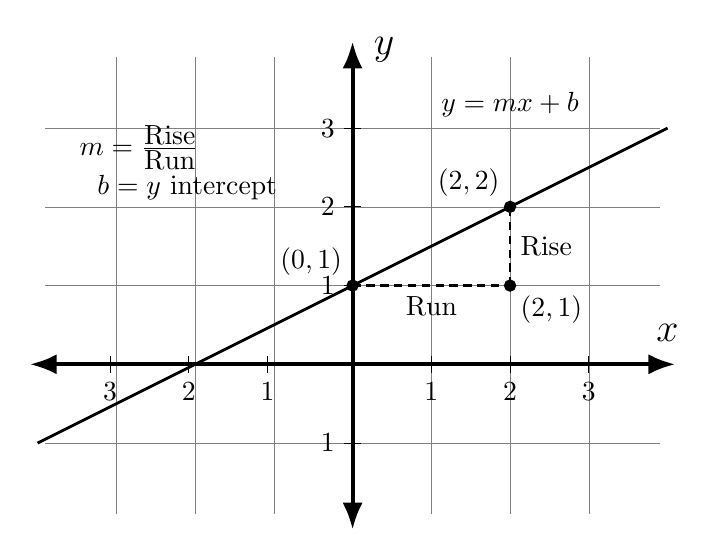
\begin{tikzpicture}[>=latex, line width=1pt]
        \draw[style=help lines] (-3.9, -1.9) grid (3.9, 3.9);
        \begin{scope}[line width=0.3pt]
            \foreach\n in {1,2,3}{%
                \draw (\n,3pt) -- (\n,-3pt) node [below] {$\n$};
                \draw (3pt,\n) -- (-3pt,\n) node [left] {$\n$};
                \draw (-\n.08,3pt) -- (-\n.08,-3pt) node [below] {$\minus\n$};
            }
            \draw (3pt,-1) -- (-3pt,-1) node [left] {$\minus{1}$};
        \end{scope}
        \begin{scope}[line width=1.5pt, >=Latex, font=\Large]
            \draw[<->] (-4.1, 0) to (4.1, 0);
            \draw[<->] (0, -2.1) to (0, 4.1);
            \node at (4, 0.4) {$x$};
            \node at (0.4, 4) {$y$};
        \end{scope}
        \draw (-4, -1) to (4, 3);
        \draw[fill=black] (0,1) circle (0.6mm) node[above left] {$(0,1)$};
        \draw[fill=black] (2,2) circle (0.6mm) node[above left] {$(2,2)$};
        \draw[fill=black] (2,1) circle (0.6mm) node[below right] {$(2,1)$};
        \draw[densely dashed] (0,1) to node [below] {Run} (2,1);
        \draw[densely dashed] (2,1) to node [right] {Rise} (2,2);
        \node at (-2.71,2.75) {$m=\frac{\textrm{Rise}}{\textrm{Run}}$};
        \node at (-2.1,2.25) {$b=y\textrm{ intercept}$};
        \node at (2,3.3) {$y=mx+b$};
    \end{tikzpicture}
\end{document}
                \caption[Example of a Line in Slope Intercept Form.]
                    {Graph of a Line with slope $m=\frac{1}{2}$ and $y$ intercept $b=1$.}
                \label{fig:Slope_Intercept_Form_001}
            \end{figure}
            \begin{lexample}{}{}
                Consider the line that passes through $(0,0)$ and $(1,1)$, and
                the line the passes through $(2,3)$ and $(\minus{1},\minus{2})$.
                Let's compute the slope, the $y$ intercept, and the root of
                these lines. First, let's graph these two.
                \begin{figure}[H]
                    \centering
                    \captionsetup{type=figure}
                    \begin{subfigure}[b]{0.49\textwidth}
                        \centering
                        \resizebox{\textwidth}{!}{\documentclass[crop,class=article]{standalone}                      %
%----------------------------Preamble-------------------------------%
\usepackage{amssymb}                                                %
\usepackage{tikz}                       % Drawing/graphing tools.   %
\usetikzlibrary{arrows.meta}            % Latex and Stealth arrows. %
\DeclareMathSymbol{\minus}{\mathbin}{AMSa}{"39} % Unary minus sign. %
%--------------------------Main Document----------------------------%
\begin{document}
    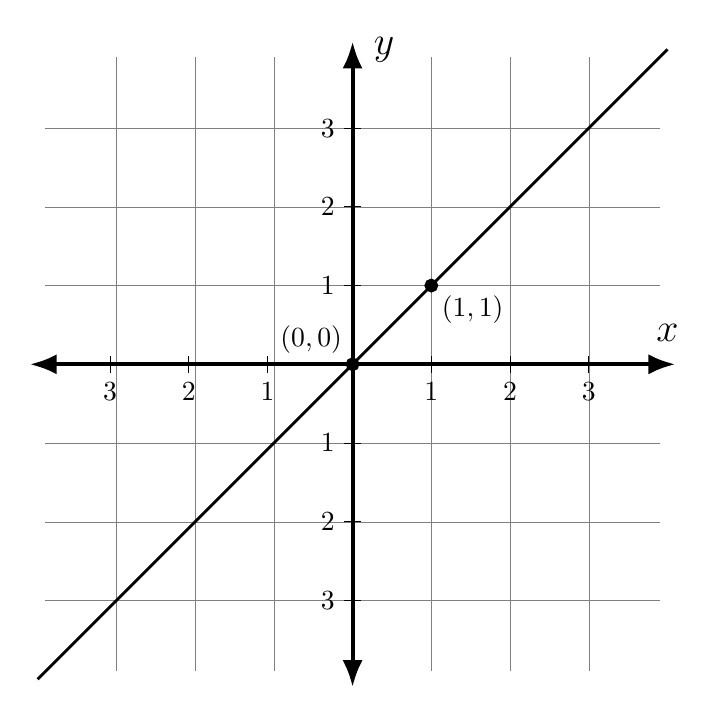
\begin{tikzpicture}[>=latex, line width=1pt]
        \draw[style=help lines] (-3.9, -3.9) grid (3.9, 3.9);
        \begin{scope}[line width=0.3pt]
            \foreach\n in {1,2,3}{%
                \draw (\n,3pt) -- (\n,-3pt) node [below] {$\n$};
                \draw (3pt,\n) -- (-3pt,\n) node [left] {$\n$};
                \draw (-\n.08,3pt) -- (-\n.08,-3pt) node [below] {$\minus\n$};
                \draw (3pt,-\n) -- (-3pt,-\n) node [left] {$\minus\n$};
            }
        \end{scope}
        \begin{scope}[line width=1.5pt, >=Latex, font=\Large]
            \draw[<->] (-4.1, 0) to (4.1, 0);
            \draw[<->] (0, -4.1) to (0, 4.1);
            \node at (4, 0.4) {$x$};
            \node at (0.4, 4) {$y$};
        \end{scope}
        \draw (-4, -4) to (4, 4);
        \draw[fill=black] (0,0) circle (0.7mm) node[above left] {$(0,0)$};
        \draw[fill=black] (1,1) circle (0.7mm) node[below right] {$(1,1)$};
    \end{tikzpicture}
\end{document}}
                        \subcaption{Graph of $y=x$}
                    \end{subfigure}
                    \begin{subfigure}[b]{0.49\textwidth}
                        \centering
                        \resizebox{\textwidth}{!}{\documentclass[crop,class=article]{standalone}
%----------------------------Preamble-------------------------------%
\usepackage{amssymb}
\usepackage[dvipsnames]{xcolor}         % Color names.
\usepackage{tikz}                       % Drawing/graphing tools.
\usetikzlibrary{arrows.meta}            % Latex and Stealth arrows.
\DeclareMathSymbol{\minus}{\mathbin}{AMSa}{"39} % Unary minus sign.
%--------------------------Main Document----------------------------%
\begin{document}
    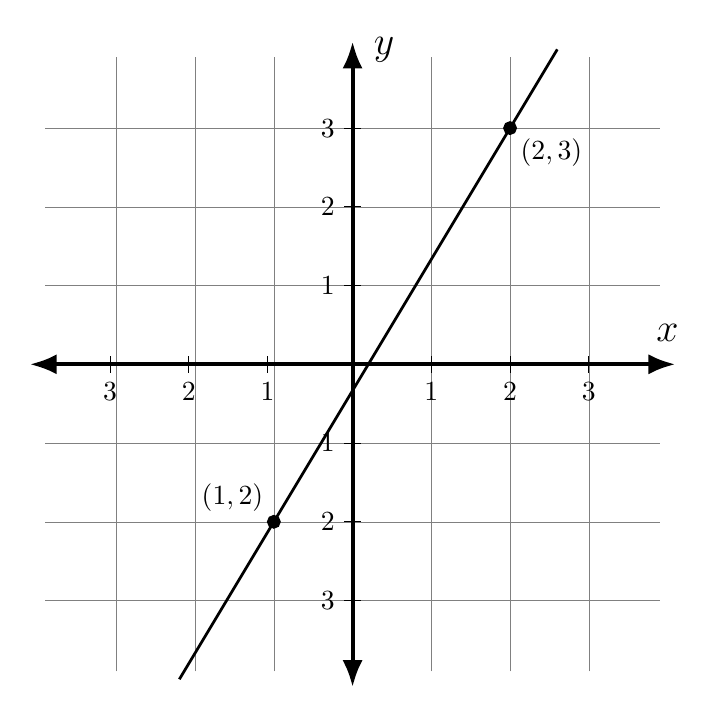
\begin{tikzpicture}[>=latex, line width=1pt]
        \draw[style=help lines] (-3.9, -3.9) grid (3.9, 3.9);
        \begin{scope}[line width=0.3pt]
            \foreach\n in {1,2,3}{%
                \draw (\n,3pt) -- (\n,-3pt) node [below] {$\n$};
                \draw (3pt,\n) -- (-3pt,\n) node [left] {$\n$};
                \draw (-\n.08,3pt) -- (-\n.08,-3pt) node [below] {$\minus\n$};
                \draw (3pt,-\n) -- (-3pt,-\n) node [left] {$\minus\n$};
            }
        \end{scope}
        \begin{scope}[line width=1.5pt, >=Latex, font=\Large]
            \draw[<->] (-4.1, 0) to (4.1, 0);
            \draw[<->] (0, -4.1) to (0, 4.1);
            \node at (4, 0.4) {$x$};
            \node at (0.4, 4) {$y$};
        \end{scope}
        \draw (-2.2, -4) to (2.6, 4);
        \draw[fill=black] (-1,-2) circle (0.7mm)
            node[above left] {$(\minus{1},\minus{2})$};
        \draw[fill=black] (2,3) circle (0.7mm) node[below right] {$(2,3)$};
    \end{tikzpicture}
\end{document}}
                        \subcaption{Graph of $y=\frac{5}{3}x-\frac{1}{3}$}
                    \end{subfigure}
                    \caption{Solutions to the First Two Problems.}
                    \label{fig:Solutions_to_First_Two_Problems}
                \end{figure}
                Using Fig.~\ref{fig:Slope_Intercept_Form_001} as our guide,
                we can compute the slope as \textit{rise} over \textit{run}.
                For the first graph, we obtain:
                \begin{equation}
                    m=\frac{1-0}{1-0}=\frac{1}{1}=1
                \end{equation}
                So the slope is $m=1$. The $y$ intercept is where the line
                crosses the $y$ axis. This occurs when $x=0$. Looking
                at the graph, we see that $b=0$. The equation of this line is:
                \begin{equation}
                    y(x)=mx+b
                    \quad\Longrightarrow\quad
                    y(x)=x
                \end{equation}
                The root is the value of $x$ such that $y(x)=0$. Since we
                have $y(x)=x$, we see that the root is simply $x=0$.
                For the points $(2,3)$ and $(\minus{1},\minus{2})$, we can again
                compute the slope and obtain:
                \begin{equation}
                    m=\frac{3-(\minus{2})}{2-(\minus{1})}
                     =\frac{3+2}{2+1}
                     =\frac{5}{3}
                \end{equation}
                To compute the $y$ intercept, we can simply plug in $x=2$
                and $y=3$:
                \begin{equation}
                    3=\frac{5}{3}(2)+b
                     =\frac{10}{3}+b
                    \quad\Longrightarrow\quad
                    b=3-\frac{10}{3}
                     =\frac{9}{3}-\frac{10}{3}
                \end{equation}
                Combining and carrying out the subtraction, we obtain:
                \begin{equation}
                    b=\frac{9}{3}-\frac{10}{3}
                    \quad\Longrightarrow\quad
                    b=\frac{9-10}{3}
                    \quad\Longrightarrow\quad
                    b=\minus\frac{1}{3}
                \end{equation}
                The slope-intercept form is thus:
                \begin{equation}
                    y=\frac{5}{3}x-\frac{1}{3}
                    \quad\Longrightarrow\quad
                    y=\frac{5x-1}{3}
                \end{equation}
                This simplified version on the right makes it simple to
                compute the root of this line. The root occurs when $y=0$.
                This can only happen if $5x-1=0$. Thus we see that the root
                is at $x=1/5$.
            \end{lexample}
            We relied on the drawing shown in
            Fig.~\ref{fig:Slope_Intercept_Form_001} to solve the problems in
            the previous example. It would be nice to have a more methodical
            and algebraic method that doesn't rely on any picture.
            Given two points in the plane, $(x_{1},y_{1})$ and $(x_{2},y_{2})$,
            we can compute the slope of the line through these two points
            as follows:
            \begin{equation}
                m=\frac{y_{2}-y_{1}}{x_{2}-x_{1}}
            \end{equation}
            Note that the order doesn't matter, since:
            \begin{equation}
                m=\frac{y_{2}-y_{1}}{x_{2}-x_{1}}
                 =\frac{(\minus{1})(y_{1}-y_{2})}{(\minus{1})(x_{1}-x_{2})}
                 =\frac{y_{1}-y_{2}}{x_{1}-x_{2}}
            \end{equation}
            And thus there's no real meaning in calling one point the
            \textit{first} and the other the \textit{second}.
            Once this is done, we have $y=mx+b$. To compute for $b$ we simply
            plug in either $x_{1}$ and $y_{1}$, or $x_{2}$ and $y_{2}$, and
            then solve for $b$. That is:
            \begin{equation}
                y_{1}=mx_{1}+b
                \quad\Longrightarrow\quad
                y_{1}-mx_{1}=b
            \end{equation}
            It would be quite upsetting if using the point $(x_{1},y_{1})$ and
            the point $(x_{2},y_{2})$ gave different answers for $b$.
            Fortunately, they yield the same answer.
            Using our equation for $m$, we obtain:
            \begin{equation}
                y_{1}-mx_{1}=y_{1}-\frac{y_{2}-y_{1}}{x_{2}-x_{1}}x_{1}
                            =y_{1}\frac{x_{2}-x_{1}}{x_{2}-x_{1}}-
                                  \frac{y_{2}-y_{1}}{x_{2}-x_{1}}x_{1}
            \end{equation}
            Since the denominators are equal, we can combine this last
            expression to obtain:
            \begin{equation}
                \frac{y_{1}(x_{2}-x_{1})-x_{1}(y_{2}-y_{1})}{x_{2}-x_{1}}
                    =\frac{y_{1}x_{2}-y_{1}x_{1}-y_{2}x_{1}+y_{1}x_{1}}
                          {x_{2}-x_{1}}
                    =\frac{y_{1}x_{2}-y_{2}x_{1}}{x_{2}-x_{1}}
            \end{equation}
            From the transitive property of equality, we have:
            \begin{equation}
                y_{1}-mx_{1}=\frac{y_{1}x_{2}-y_{2}x_{1}}{x_{2}-x_{1}}
            \end{equation}
            We can repeat this $y_{2}$ and $x_{2}$, to obtain:
            \begin{equation}
                y_{2}-mx_{2}=y_{2}-\frac{y_{2}-y_{1}}{x_{2}-x_{1}}x_{2}
                            =y_{2}\frac{x_{2}-x_{1}}{x_{2}-x_{1}}-
                                  \frac{y_{2}-y_{1}}{x_{2}-x_{1}}x_{2}
            \end{equation}
            Further simplifying, we have:
            \begin{equation}
                \frac{y_{2}(x_{2}-x_{1})-x_{2}(y_{2}-y_{1})}{x_{2}-x_{1}}
                    =\frac{y_{2}x_{2}-y_{2}x_{1}-y_{2}x_{2}+y_{1}x_{2}}
                          {x_{2}-x_{1}}
                    =\frac{y_{1}x_{2}-y_{2}x_{1}}{x_{2}-x_{1}}
            \end{equation}
            Piecing this together, we have found that:
            \begin{equation}
                b=y_{1}-mx_{1}
                 =\frac{y_{1}x_{2}-y_{2}x_{1}}{x_{2}-x_{2}}
                 =y_{2}-mx_{2}
            \end{equation}
            And thus it doesn't matter which point we choose when calculating
            $b$.
            \newpage
            \begin{problem}
                Given the following two points in the plane,
                graph the line that passes through these, compute
                the slope and $y$ intercept, and find the root.
                Then give the equation of the line in slope-intercept
                form.
                \begin{enumerate}
                    \begin{multicols}{3}
                        \item $(2,0)$, $(3,1)$
                        \item $(\minus{1},\minus{2})$, $(\frac{1}{2},2)$
                        \item $(1,1)$, $(3,1)$
                        \item $(\frac{3}{4},\frac{2}{3})$, $(\frac{5}{2},2)$
                        \item $(\sqrt{2},\sqrt{3})$, $(\sqrt{8},\sqrt{12})$
                        \item $(0,\pi)$, $(\minus{1},0)$
                        \item $(1,2)$, $(1,3)$
                    \end{multicols}
                \end{enumerate}
            \end{problem}
            \begin{lexample}{}{}
                A line is uniquely determined by two points in the plane.
                Thus, given the point $(1,1)$ and the point $(2,3)$, it is
                possible to compute the equation of the line that passes through
                these. We note that a straight-line is a one dimensional object
                and thus it seems reasonable to suspect that we can determine
                all of the points with the use of a single variable. It is
                somewhat standard to use the Greek letter \textit{lambda}, or
                the letter $t$, as our single parameter. To make things simple,
                let's try to find a parameter $t$ such that when $t=0$ we get
                the point $(1,1)$, and when $t=1$ we get the point $(2,3)$.
                There's a straight-forward way to do this:
                \begin{equation}
                    \Gamma(t)=t\big(2,3\big)+(1-t)\big(1,1\big)
                \end{equation}
                If we plug in $t=0$, the point $(2,3)$ get's zeroed out, and
                we are left with $(1,1)$. Evaluating $t=1$, we see that
                $1-t=0$, and thus the $(1,1)$ point is discarded, so we are
                left with $(2,3)$. To see that this is the equation of a
                straight line, note that we can rewrite this as:
                \begin{equation}
                    \Gamma(t)=(1,1)+t\big((2,3)-(1,1)\big)
                             =(1,1)+t\big(1,2\big)
                \end{equation}
                Given the following two points in the plane,
                graph the line that passes through these, compute
                the slope and $y$ intercept, and find the root.
                Then give the equation of the line in slope-intercept
                form.
            \end{lexample}
        \begin{problem}
            The general equation for a line is:
            \begin{equation}
                \label{eqn:general_line}%
                Ax+By+C=0
            \end{equation}
            This is contrasted with the slope-intercept form:
            \begin{equation}
                \label{eqn:slope_intercept_form}%
                y=mx+b
            \end{equation}
            Find an example of a line that can be written
            in the form of Eqn.~\ref{eqn:general_line} but
            cannot be written in the form of
            Eqn.~\ref{eqn:slope_intercept_form}. Draw the graph of
            this line.
            \par
            Hint: Consider the line the passes through
            $(1,1)$ and $(3,1)$. What's special about this line?
            Can it be written in the form of
            Eqn.~\ref{eqn:general_line}? What about
            Eqn.~\ref{eqn:slope_intercept_form}?
        \end{problem}
        \newpage
        \begin{problem}
            Solve the following systems of linear equations.
            Determine if there is one solution, infinitely many
            solutions, or no solutions. Graph the lines as well.
            \begin{align*}
                (1)\quad{y}&=3x+2&(2)\quad{3}y&=6x+6\\
                2y&=4x+8&y&=2x+2\\
                \hfill\\
                (3)\quad{2}y&=3x+3&(4)\quad{2}y&=2x+1\\
                4y&=6x+7&3y&=x-6
            \end{align*}
        \end{problem}
        \begin{align*}
            2y-3x&=3\\
            4y-6x&=7
        \end{align*}
        \par\hfill\par
        \begin{align*}
            \minus{3}x+2y&=3\\
            \minus{6}x+4y&=7
        \end{align*}
        \par\hfill\par
        \begin{equation}
            \begin{pmatrix}
                \minus{3}&2\\
                \minus{6}&4
            \end{pmatrix}
            \begin{pmatrix}
                x\\y
            \end{pmatrix}
            =
            \begin{pmatrix}
                3\\7
            \end{pmatrix}
        \end{equation}
        \begin{equation}
            \begin{pmatrix}
                x\\y
            \end{pmatrix}
            =
            \begin{pmatrix}
                a&b\\
                c&d
            \end{pmatrix}
            \begin{pmatrix}
                3\\7
            \end{pmatrix}
        \end{equation}
        \begin{equation}
            \begin{bmatrix}
                \minus{3}&2&\vline&1&0\\
                \minus{6}&4&\vline&0&1
            \end{bmatrix}
        \end{equation}
        \begin{example}
            The set of all quadratic polynomials in one variable is a family
            of equations. So is the set of all polynomials in three variables.
        \end{example}
        We wish to study the family of linear equations of one variable. These have the form $y=mx+b$.
        \begin{definition}
        An equations is a statement that two expressions are equal.
        \end{definition}
        We've already seen plenty of equations in the preliminaries section. There are many arithmetic properties that equations have.
        \begin{properties}[Properties of Equality]
        If $A,B,$ and $C$ are algebraic expressions, then:
        \begin{enumerate}
        \item If $A=B$, then $A+C=B+C$ for all $C$. \hfill [Additive Property of Equality]
        \item If $A=B$, then $A\cdot C = B\cdot C$ \hfill [Multiplicative Property of Equality]
        \item If $C \ne 0$, and $A=B$, then $\frac{A}{C} = \frac{B}{C}$ \hfill [Division Property of Equality]
        \item If $C\ne 0$, and $A\cdot C = B\cdot C$, then $A=B$. \hfill [Cancellation Law of Equality]
        \end{enumerate}
        \end{properties}
        \begin{remark}
        Note that $A\cdot C = B\cdot C$ is not enough to say that $A=B$. If $C = 0$, then $2\cdot 0 = 0$ and $5\cdot 0 = 0$, so $2\cdot 0 = 5\cdot 0$, but $2\ne 5$. If $C = 0$, then we can say that $A=B$.
        \end{remark}
        \begin{example}
        Solve for $x$: $3(x-1) +x = -x+7$. We have $3x-3+x = 4x-3 = -x+7$. Adding $x$ to both sides, $\big(4x-3)+x = \big(-x+7)+x$. So $5x-3 = 7$. Adding $3$ to both sides, $\big(5x-3\big)+3 = 7+3$, so $5x = 10$. Dividing by $5$, we get $x = \frac{10}{5} = 2$.
        \end{example}
        \begin{example}
        Solve for for $n$: $\frac{1}{4}\big(n+8\big) = \frac{1}{2}\big(n-6\big)$: Multiplying both sides by $4$, we have $(n+8)-8 = 2(n-6)$, so $n = 2n-12$. Subtracting $2n$ from both sides, we get $-n = -12$. Multiplying both sides by $-1$, we get $n=12$.
        \end{example}
        The two previous examples are examples of conditional equations.
        \begin{definition}
        A conditional equation is an equation that is only true for certain values of the variables involved in the equation.
        \end{definition}
        \begin{definition}
        An identity is an equation that is true of all values of the variables in the equation.
        \end{definition}
        \begin{example}
        $2x + 4 = 2(x+2)$ is an identity. It is true of all values of $x$.
        \end{example}
        \begin{example}
        $\sqrt{x^2}=|x|$ is an identity. It is true of all values of $x$.
        \end{example}
        \begin{definition}
        A contradiction is an equation that is never true, regardless of the value the variables may take.
        \end{definition}
        \begin{example}
        $x=x+1$ is a contradiction. For $x = x+1$ implies $0=1$, which is false.
        \end{example}
        \begin{example}
        $2x - 5 = 2x$ is a contradiction. This would imply $0=5$, which is false.
        \end{example}
        \begin{definition}
        A literal equation is an equation involving more than one variable.
        \end{definition}
        \begin{example}
        The ideal gas law states that $PV=nRT$, where $P$ is the pressure, $V$ is the volume, $n$ is the number of moles in the system, and $T$ is the temperature. $R$ is a constant known as the universal gas constant. This is a literal equation in $4$ variables ($R$ is not a variable, it is a set constant). Solving for $P$, we get $P = \frac{nRT}{V}$.
        \end{example}
        \begin{example}
        The amount of money $A$ earned from a simple interest model is $A = A_0+A_0Rt$, where $A_0$ is the initial deposit, $R$ is the
        interest rate, and $t$ is the time elapsed since the deposit. Solve for $A_0$ in terms of $A,R,$ and $t$.
        $A_{0}(1+Rt)=A$, so $A_{0}=\frac{A}{1+Rt}$
        \end{example}
        \begin{theorem}[General Solution to a Linear Equation]
        If $a,b,c,d\in \mathbb{R}$, $a,c, \ne 0$, then:
        \begin{enumerate}
        \item If $ax+b=0$, then $x=-\frac{b}{a}$
        \item If $ax+b=d$, then $x=\frac{c-b}{a}$
        \item If $ax+b=cx+d$, and $a\ne c$, then $x =\frac{d-b}{a-c}$
        \end{enumerate}
        \end{theorem}
        \begin{remark}
        $ax+b=c$ is a linear equation in $x$. That is, it does not involve higher powers of $x$ ($x^{2},x^{3}$, etc.). It is a literal
        equation, as $a$, $b$ and $c$ can be any real number (So long as $a\ne 0$), but we only care about solutions for $x$.
        \end{remark}
        \begin{example}
            Give a formula for the sum of three consecutive integers. Let $n$ be the smallest integer. The next integer is $n+1$, and the one
            thereafter if $n+2$. We are summing them, so we have $n+(n+1)+(n+2)$. From the associative and commutative properties of addition,
            we have $(n+n+n)+(1+2)=3n+3=3(n+1)$. So the sum of three consecutive integers, starting at $n$, is $3(n+1)$.
        \end{example}
        \subsubsection{Solved Problems}
        \begin{enumerate}
            \begin{multicols}{2}
                \item $4x+3(x-2)=18-x:x=3$
                \item $15-2x=9-4(x+1):x=-5$
                \item $21-(2x+17)=-(7-x):x=-11$
                \item $12+5x=9+(6x+7):x=-4$
                \item $-3(4x+5)=-15x-20+3x:$ Contradiction.
                \item $5x-9-2=-5(2-x)-1:$ Identity
                \item $8-8(3x+5)=-5+6(x+1):x=-\frac{11}{10}$
                \item $-4(4x+5)=-6-2(8x+7):$ Identity
            \end{multicols}
        \end{enumerate}
        \subsubsection{Linear Inequalities in One Variable}
        \begin{definition}
        A linear inequality in one variable is an inequality involving two linear expressions in one variable.
        \end{definition}
        \begin{definition}
        The solution set to an inequality is the set of real numbers that satisfy the inequality.
        \end{definition}
        \begin{example}
        $x +1 > 5$ has the solution set $\{x:x>4\}$. That is, all real numbers greater than $4$.
        \end{example}
        \begin{notation}
        The following notations are used to represents intervals of the real line. Let $a,b\in\mathbb{R}$, $a<b$:
            \begin{enumerate}
                \item $(a,\infty)=\{x:a<x<\infty\}$\hfill[Open Right-Half Line
                \item $[a,\infty)=\{x:a\leq x<\infty\}$\hfill[Closed Right-Half Line]
                \item $(a,b)=\{x:a<x<b\}$\hfill[Open Interval]
                \item $[a,b)=\{x:a\leq x<b\}$\hfill[Right Semi-Open Interval]
                \item $(a,b]=\{x:a<x\leq b\}$\hfill [Left Semi-Open Interval]
                \item $[a,b]=\{x:a\leq x\leq b\}$\hfill[Closed Interval]
                \item $(-\infty,b]=\{x:x\leq b\}$\hfill[Closed Left-Half Line]
                \item $(-\infty,b)=\{x:x<b\}$\hfill[Open Left-Half Line]
            \end{enumerate}
        \end{notation}
        \begin{properties}[Properties of Inequalities]
        If $a<b$, $c\in\mathbb{R}$, then the following are true:
        \begin{enumerate}
            \item $a+b<b+c$ \hfill [Additive Property of Inequalities]
            \item If $c>0$, then $a\cdot c<b\cdot c$ \hfill [Multiplicative Property of Inequalities]
            \item $-b<-a$ \hfill [Negation Property of Inequalities]
        \end{enumerate}
        \end{properties}
        \begin{example}
        $1<2$, and $1-5=-4<2-5=-3$. Also $\pi>0$, and thus $\pi\cdot 1<\pi\cdot 2$. We know that $3<4$, but multiplying
        by $-1$ flips the inequality, and we get $-4<-3$ (Or $-3>-4)$.
        \end{example}
        \begin{definition}
        A compound inequality is an inequality where the solution set is multiple intervals.
        \end{definition}
        \begin{example}
        $-3x-1<-4$ or $4x+3<-6$. This has the requirement that $x>1$ or $x< -\frac{9}{4}$. To write this in interval notation,
        we do $(-\infty,-\frac{9}{4})\cup (1,\infty)$
        \end{example}
        \begin{example}
        $3x+5>-13$ and $3x+5<-1$. This has the requirement that $x>-6$ and $x<-2$. In interval notation,
        we have $(-6,\infty)\cap (-\infty,-2)=(-6,-2)$.
        \end{example}
        \begin{example}
        Solve $-6\leq\frac{2x+5}{-3}<1$. Multiplying by $-3$, we must flip the inequality to get $-3<2x+5\leq 18$.
        Subtracting $5$, we have $-8<2x\leq 13$. Dividing by $2$, we have $-4 <x \leq\frac{13}{2}$. In interval notation,
        that $(-4,\frac{13}{2}]$.
        \end{example}
        \begin{definition}
        The domain of an expression is the set of values for which the expression is well defined.
        \end{definition}
        \begin{example}
        $\frac{1}{x}$ is undefined at $0$, so its domain is $(-\infty, 0)\cup (0,\infty)$.
        \end{example}
        \begin{remark}
        Remember from interval notation that $(-\infty,0)\cup (0,\infty)$ does not include the number $0$. It includes every
        real number except for $0$.
        \end{remark}
        \subsubsection{Solved Problems}
        Determine the domain of the following expressions in interval notation:
        \begin{enumerate}
            \begin{multicols}{2}
                \item $\frac{12}{x}:(-\infty,0)\cup(0,\infty)$
                \item $\frac{5}{x+7}:(-\infty,-7)\cup(-7,\infty)$
                \item $\frac{1}{x-7}:(-\infty,7)\cup(7,\infty)$
                \item $\frac{4}{x-3}:(-\infty,3)\cup(3,\infty)$
            \end{multicols}
        \end{enumerate}
        \subsubsection{Absolute Value Equations and Inequalities}
        Inequalities can involve the absolute value of a variable. When this happens, we must be careful when solving for the solution set.
        \begin{properties}[Properties of Absolute Value Inequalities]
        If $A$ and $B$ are algebraic expressions and $a>0$, then:
            \begin{enumerate}
                \item $|A|=a$ if and only if either $A=a$, or $A=-a$.
                \item $|A|>a$ if and only if either $A>a$ or $-A>a$
                \item $|A|<a$ if and only if $-a<A<a$
                \item $|A\cdot B|=|A|\cdot|B|$
            \end{enumerate}
        \end{properties}
        \begin{example}[Examples of Absolute Values in Inequalities]
        \
            \begin{enumerate}
                \item $-5|x-7|+2=-13$ is equivalent to $|x-7|=-15$, and so $x-7=3$ or $x-7=-3$. The solution set is $\{4,10\}$.
                \item $|5-2x|=7$ implies either $5-2x=7$, or $5-2x=-7$. The solution set is $\{-1,6\}$.
                \item $|x|<7$ implies $-7<x<7$. The solution set is the interval $(-7,7)$.
                \item $|x-2|<7$ implies $-5<x<9$. The solution set is $(-5,9)$.
                \item $|x+1|>4$ implies $x+1>4$ or $x+1<-4$. The solution set is $(-\infty, -5)\cup (3,\infty)$
            \end{enumerate}
        \end{example}
        \subsubsection{Solved Problems}
        Find the solution sets. Write the answer in set notation or using interval notation.
        \begin{enumerate}
            \begin{multicols}{3}
                \item $2|x-1|-7=3:\{-4,6\}$
                \item $3|x-5|-14=-2:\{1,9\}$
                \item $-3|x+5|+6=-15:\{2,-12\}$
                \item $|x|=1:\{-1,1\}$
                \item $|x-2|\leq 7:[-5,9]$
                \item $|x-2|<7:(-5,9)$
                \item $5|x-2|-7\leq 8:[-1,5]$
                \item $-|x| > 2:\emptyset$
                \item $-|x|<1:\mathbb{R}$
            \end{multicols}
        \end{enumerate}
        \subsubsection{Complex Numbers}
        There is no real number $x\in \mathbb{R}$ such that $x^2 = -1$. That's because the square of a real number is either zero, or
        positive. In fact, $0$ is the only solution to $x^2 = 0$. Thus, every other real number has that property that its square is
        positive. Solving the equation $x^2+1 = 0$ doesn't make sense in the realm of real numbers, and up until now we'd simply say
        there is no solution. That is, there is no such thing is $\sqrt{-1}$. To solve this problem, we introduce imaginary and
        complex numbers.
        \begin{definition}
        The imaginary unit $i$ is a number such that $i^{2}=-1$.
        \end{definition}
        \begin{remark}
        Note that the imaginary unit is not a real number (Hence the name). It is a part of the larger complex numbers.
        \end{remark}
        \begin{notation}
        If $r$ is a positive real number, we write $\sqrt{-r}=i\sqrt{r}$.
        \end{notation}
        \begin{remark}
        Note that if $r$ is a negative real number, then $\sqrt{-r}=\sqrt{|r|}$, which is a real number.
        \end{remark}
        \begin{definition}
        The principle square root of a negative real number $r$, is the complex number $i\sqrt{|r|}$.
        \end{definition}
        \begin{definition}
        A complex number is a sum $a+ib$, where $a$ and $b$ are real numbers, and $i$ is the imaginary unit.
        \end{definition}
        \begin{definition}
        The set of all complex number, denoted $\mathbb{C}$, is the set $\{a+ib:a,b\in \mathbb{R}\}$.
        \end{definition}
        \begin{example}[Examples of Complex Numbers]
        \
        \begin{enumerate}
            \begin{multicols}{4}
                \item $4+\sqrt{-49}=4+7i$
                \item $1-\sqrt{-1}=1-i$
                \item $25+\sqrt{-16}=25+4i$
                \item $1-\sqrt{-100}=1-10i$
            \end{multicols}
        \end{enumerate}
        \end{example}
        \begin{remark}
        Note that from the definition of complex numbers, $\mathbb{R}\subset \mathbb{C}$.
        \end{remark}
        The sum and difference of complex numbers is computed using the distributive property to group purely imaginary and purely
        real components together. We multiply using the distributive property and the fact that $i^{2}=-1$.
        \begin{example}[Examples of Complex Arithmetic]
        \
        \begin{enumerate}
            \begin{multicols}{4}
                \item $(2+3i)+(1+i)=3+4i$
                \item $(1+i)+(1-i)=2$
                \item $(1+i)(1-i)=1-i^{2}=1-(-1)=2$
                \item $i(2+3i)=-3+2i$
            \end{multicols}
        \end{enumerate}
        \end{example}
        \begin{remark}
        The powers of $i$ go in a cycle:
        \begin{enumerate}
            \begin{multicols}{4}
                \item $i^{1}=i$
                \item $i^{2}=-1$ 
                \item $i^{3}=i\cdot i^{2}=-i$
                \item $i^{4}=i^{2}\cdot i^{2}=1$
                \item $i^{5}=i^{4}\cdot i=i$
                \item $i^{6}=i^{4}\cdot i^{2}=-1$
                \item $i^{7}=i^{4}\cdot i^{3}=-i$
                \item $i^{8}=i^{4}\cdot i^{4}=1$
            \end{multicols}
        \end{enumerate}
        \end{remark}
        \begin{example}[Simplifying Powers of $i$]
        \
        \begin{enumerate}
            \begin{multicols}{3}
                \item $i^{22}=\big(i^{4}\big)^{5}\cdot i^{2}=1\cdot i^{2}=-1$
                \item $i^{57}=\big(i^{4}\big)^{14}\cdot i=1\cdot i=i$
                \item $i^{75}=\big(i^{4}\big)^{18}\cdot i^{3}=1\cdot i^{3}=i^{3}$
            \end{multicols}
        \end{enumerate}
        \end{example}
        \begin{definition}
        The complex conjugate of a complex number $z=a+ib$, denoted $\overline{z}$, is the complex number $\overline{z} = a-ib$.
        \end{definition}
        \begin{remark}
        For a real number $z$, $\overline{z}=z$. This is because if $z=a+ib$ is real, then $b=0$.
        \end{remark}
        \begin{theorem}[The Complex Conjugate Theorem]
        If $z=a+ib$ is a complex number, then $z\cdot\overline{z}=a^{2}+b^{2}$
        \end{theorem}
        \begin{proof}
        For $z\cdot\overline{z}=(a+ib)(a-ib)=a^{2}+iab-iab-(ib)^{2}=a^{2}-(i)^{2}b^{2}=a^{2}+b^{2}$
        \end{proof}
        While $x^{2}+y^{2}$ cannot be simplified, in general, over the real numbers, it can by factored over the complex numbers.
        If $x$ and $y$ are real numbers, then $x^{2}+y^{2}=(x+iy)(x-iy)$. This is just an application of the complex conjugate theorem.
        We define division the following way: If $z=a+ib$, $w=c+id$, where $c,d\ne 0$, then
        $\frac{z}{w}=\frac{z\cdot\overline{w}}{w\cdot\overline{w}}=\frac{(ac-bd)+i(ad+cb)}{c^{2}+d^{2}}$
        \begin{example}[Examples of Division by Complex Numbers]
        \
        \begin{enumerate}
            \begin{multicols}{3}
                \item $\frac{2}{5-i}=\frac{5+i}{13}$
                \item $\frac{3-i}{2+i}=1-i$
                \item $\frac{6+6i}{3+3i}=2$
            \end{multicols}
        \end{enumerate}
        \end{example}
        \subsubsection{Solved Problems}
        \begin{enumerate}
            \begin{multicols}{3}
                \item $\sqrt{-16}=4i$
                \item $\sqrt{27}=3\sqrt{3}$
                \item $\sqrt{-81}=9i$
                \item $-\sqrt{-64}=-8i$
                \item $\sqrt{-49}=7i$
                \item $\sqrt{|-25|}=5$
                \item $\sqrt{-17}=i\sqrt{17}$
                \item $\sqrt{-\frac{9}{16}}=\frac{3}{4}i$
                \item $(12-2i)+(7+3i)=19+i$
                \item $(14+i)-(7+3i)=7-2i$
                \item $5+(1-i)=6-i$
                \item $(2+2i)+(-5-i)=-3+i$
                \item $(1+i)(2+i)=1+3i$
                \item $(4+i)(4-i)=17$
                \item $i(6-17i)=17+6i$
                \item $\frac{1+i}{1-i}=i$
                \item $i^{2}7=i^{3}$
                \item $i^{81}=i$
            \end{multicols}
        \end{enumerate}
        \subsubsection{Solving Quadratic Equations}
        \begin{definition}
        A quadratic equation is an equation of the form $ax^{2}+bx+c=0$, where $a,b,c\in\mathbb{R}$, and $a\ne 0$.
        \end{definition}
        \begin{remark}
        All quadratic equations have degree $2$. The highest power that occurs is $x^{2}$, hence they are degree $2$.
        \end{remark}
        Quadratic equations often have two solutions, whereas linear equations have only one. There is a property of real numbers
        that allows us to solve quadratic equations, called the Euclidean Property of Real Numbers.
        \begin{properties}[The Euclidean Property of Real Numbers]
        \
        \begin{enumerate}
        \item If $a,b\in \mathbb{R}$ and $a\cdot b = 0$, then either $a=0$ or $b=0$, or both.
        \end{enumerate}
        \end{properties}
        \begin{remark}
        This says that if the product of two numbers is zero, one of these numbers must be zero. It is named after Euclid of Alexandria,
        one of the greatest mathematicians to ever live, who proved this in the context of geometry around $300$ B.C.
        \end{remark}
        \begin{example}
        Solve $x^{2}=x$. We have that $x^{2}-x=0$, and thus $x(x-1)=0$. From the Euclidean property, either $x=0$ or $x-1=0$.
        Thus, the solutions are $x=0$ and $x=1$.
        \end{example}
        \subsubsection{Completing the Square}
        Recall that $(x+y)^2 = x^2+2xy+y^2$. Given $ax^2+bx+c$, we can reverse this process to obtain a simplified version. This process is called completing the square. Note that $ax^2+bx = a\big(x^2+\frac{b}{a}x\big) = a\big[\big(x+\frac{b}{2a}\big)^2-\frac{b^2}{4a^2}\big]$. So, $ax^2+bx+c = a\big[\big(x+\frac{b}{2a}\big)^2 - \frac{b^2}{4a^2}\big] + c$. Solving for $ax^2+bx+c=0$ is thus equivalent to solving $a\big[\big(x+\frac{b}{2a}\big)^2-\frac{b^2}{4a^2}\big]+c=0$. We get $\big(x+\frac{b}{2a}\big)^2=\frac{b^2}{4a^2} -\frac{c}{a} = \frac{b^2-4ac}{4a^2}$. Taking square roots, we have $x+\frac{b}{2a} = \pm\frac{\sqrt{b^2 - 4ac}}{2a}$, where $\pm$ means 'Plus or Minus.' Meaning both the $+$ symbol in front or the $-$ symbol in front yield correct answers. Finally, we get $x = \frac{-b\pm \sqrt{b^2-4ac}}{2a}$. With this, we have solved every quadratic equation possible (Remember for it to be quadratic $a$ cannot equal $0$).
        \begin{theorem}[The Quadratic Formula]
            If $a,b,c\in\mathbb{R}$, $a\ne 0$, and $ax^{2}+bx+c=0$, then the solution set is
            $\{\frac{-b-\sqrt{b^{2}-4ac}}{2a},\frac{-b+\sqrt{b^{2}-4ac}}{2a}\}$
        \end{theorem}
        \begin{remark}
        It is possible that the solution to a quadratic is complex or purely imaginary. This occurs when $b^{2}-4ac<0$ 
        \end{remark}
        \begin{definition}
        The discriminant of a quadratic $ax^{2}+bx+c$ is the number $b^{2}-4ac$
        \end{definition}
        The discriminant has a useful property.
        \begin{theorem}
            If $a,b,c\in\mathbb{R}$, $a\ne 0$, and $ax^{2}+bx+c=0$, then:
            \begin{enumerate}
                \item There are no real solutions is $b^{2}-4ac<0$
                \item There is one real solution if $b^{2}-4ac=0$
                \item There are two real solutions if $b^{2}-4ac>0$
            \end{enumerate}
        \end{theorem}
        By considering the discriminant, we can determine how many real solutions there are without having to solve the quadratic.
        \subsubsection{Order of Operations}
            We start with the fundamental properties of
            addition, multiplication, and exponentiation.
            \begin{properties}[Arithmetic Properties]
                \label{property:North_Shore_Arithmetic_Properties}
                \
                \begin{enumerate}
                    \item
                        \label{%
                            property:%
                            North_Shore_Arithmetic_Properties_%
                            Com_Add%
                        }
                        $a+b=b+a$\hfill
                        [Commutativity of Addition]
                    \item
                        \label{
                            property:%
                            north_shore_arithmetic_properties_%
                            assoc_add%
                        }
                        $a+(b+c)=(a+b)+c$\hfill
                        [Associativity of Addition]
                    \item
                        \label{%
                            property:%
                            north_shore_arithmetic_properties_%
                            comm_mult%
                        }
                        ${a}\cdot{b}={b}\cdot{a}$\hfill
                        [Commutativity of Multiplication]
                    \item
                        \label{%
                            property:%
                            north_shore_arithmetic_properties_%
                            assoc_mult%
                        }
                        ${a}\cdot{({b}\cdot{c})}%
                         ={({a}\cdot{b})}\cdot{c}$\hfill
                        [Associativity of Multiplication]
                    \item
                        \label{%
                            property:%
                            north_shore_arithmetic_properties_%
                            add_identity
                        }
                        $a+0=a$\hfill%
                        [Identity Property of Addition]
                    \item
                        \label{%
                            property:%
                            north_shore_arithmetic_properties_%
                            mult_identity%
                        }
                        ${a}\cdot{1}=a$\hfill
                        [Identity Property of Multiplication]
                    \item
                        \label{%
                            property:%
                            north_shore_arithmetic_properties_%
                            add_inverse%
                        }
                        $a+(-a)=0$\hfill
                        [Inverse Property of Addition]
                    \item
                        \label{%
                            property:%
                            north_shore_arithmetic_properties_%
                            mult_inverse%
                        }
                        If ${a}\ne{0}$, then $\frac{a}{a}=1$\hfill
                        [Inverse Property of Multiplication]
                    \item
                        \label{%
                            property:%
                            north_shore_arithmetic_properties_%
                            distributive_property%
                        }
                        ${a}\cdot{(b+c)}%
                         ={a}\cdot{b}+{a}\cdot{c}$\hfill
                        [Distributive Property of
                         Multiplication over Addition]
                \end{enumerate}
            \end{properties}
            \begin{properties}[Properties of Exponents]
                \
                \label{property:North_Shore_Exponent_Rules}
                \begin{enumerate}
                    \item
                        \label{%
                            property:%
                            north_shore_distributive_property_%
                            of_expo%
                        }
                        $({x}\cdot{y})^{n}%
                         ={x^{n}}\cdot{y^{n}}$\hfill
                        [Distributive Property of Exponents]
                    \item
                        \label{%
                            property:%
                            north_shore_inverse_property_of_expo%
                        }
                        $x^{-n}=\frac{1}{x^n}$\hfill
                        [Inverse Property of Exponents]
                    \item
                        \label{%
                            property:%
                            north_shore_power_property_of_expo%
                        }
                        $(x^n)^{m}=x^{{n}\cdot{m}}$\hfill
                        [Power Property of Exponents]
                    \item
                        \label{%
                            property:%
                            north_shore_product_property_of_expo%
                        }
                        $x^{n}x^{m}=x^{n+m}$\hfill
                        [Multiplicative Property of Exponents]
                \end{enumerate}
            \end{properties}
            The order of operations \gls{pemdas} tells one
            how to simplify expressions.
            \begin{enumerate}
                \label{North_Shore_PEMDAS}
                \item \textbf{P}arenthesis.
                \item \textbf{E}xponents.
                \item \textbf{M}ultiplication or \textbf{D}ivision, 
                    in the order they appear from left to right.
                \item \textbf{A}ddition or \textbf{S}ubtraction,
                    in the order they appear from left to right.
            \end{enumerate}
            \begin{fexample}{}{}
                \begin{enumerate}
                    \item ${2}\cdot{3}+{4}\cdot{5}%
                           \overset{\textrm{\tiny{M}}}{=}%
                           6+20\overset{\textrm{\tiny{A}}}{=}%
                           \boxed{26}$
                    \item ${2}\cdot{3}%
                           +4\overset{\textrm{\tiny{M}}}{=}%
                           6+4\overset{\textrm{\tiny{A}}}{=}%
                           \boxed{10}$
                    \item ${3}\cdot{3+2^{4}}%
                           \overset{\textrm{\tiny{E}}}{=}%
                           {3}\cdot {3}+16%
                           \overset{\textrm{\tiny{M}}}{=}%
                           9+16\overset{\textrm{\tiny{A}}}{=}%
                           \boxed{25}$
                    \item $(4+1)^2-17\cdot 3%
                        \overset{\textrm{\tiny{P}}}{=}%
                        5^{2}-17\cdot 3%
                        \overset{\textrm{\tiny{E}}}{=}25-17\cdot 3%
                        \overset{\textrm{\tiny{M}}}{=}25-51%
                        \overset{\textrm{\tiny{S}}}{=}\boxed{-26}$
                    \item ${(1+1)^{(2+3)}\cdot}{5}-%
                           {2}\cdot{3}
                           \overset{\textrm{\tiny{P}}}{=}%
                           {2^{5}}\cdot{5}-{2}\cdot{3}%
                           \overset{\textrm{\tiny{E}}}{=}%
                           {32}\cdot{5}-{2}\cdot{3}%
                           \overset{\textrm{\tiny{M}}}{=}%
                           160-6\overset{\textrm{\tiny{S}}}{=}%
                           \boxed{154}$
                    \item $(2+2)-(16-11)^{(1+1)}%
                           \overset{\textrm{\tiny{P}}}{=}4-5^{2}%
                           \overset{\textrm{\tiny{E}}}{=}4-25%
                           \overset{\textrm{\tiny{S}}}{=}%
                           \boxed{-21}$
                \end{enumerate}
            \end{fexample}
            Many problems involve radicals and exponents.
            These are defined by:
            \begin{align*}
                \sqrt{x}&=x^{\frac{1}{2}}
                &
                \sqrt[n]{x}&=x^{\frac{1}{n}}
                &
                \sqrt[n]{x^m}&=x^{\frac{m}{n}}
            \end{align*}
            \begin{fexample}{}{}
                \begin{enumerate}
                    \begin{multicols}{4}
                        \item $\sqrt{x}=x^{\frac{1}{2}}$
                        \item $\sqrt[3]{x}=x^{\frac{1}{3}}$
                        \item $\sqrt[5]{x}=x^{\frac{1}{5}}$
                        \item $\sqrt[27]{x}=x^{\frac{1}{27}}$
                        \item $\sqrt{x^3}=x^{\frac{3}{2}}$
                        \item $\sqrt[3]{x^2}=x^{\frac{2}{3}}$
                        \item $\sqrt[15]{x^3}=x^{\frac{1}{5}}$
                        \item $\sqrt[3]{x^3}=x$
                    \end{multicols}
                \end{enumerate}
            \end{fexample}
            There are several theorems that help one simplify
            equations involving radicals and exponents.
            \begin{ftheorem}{Radical Formulas}{North_Shore_Radical_Formulas}
                \begin{enumerate}
                    \item If $a$ and $b$ are \textbf{positive} real numbers,
                          then $\sqrt{{a}\cdot{b}}=\sqrt{a}\cdot\sqrt{b}$
                    \item If $x$ is \textbf{positive} and $i$ is the
                          imaginary unit $(i^{2}=-1)$, then $\sqrt{-x}=i\sqrt{x}$
                    \item If $n$ is an \textbf{odd} integer
                          and $x$ is a \textbf{real} number,
                          then $\sqrt[n]{-x}=-\sqrt[n]{x}$
                    \item If $x\ne{0}$, then $x^{0}=1$. $0^{0}$ is undefined.
                \end{enumerate}
            \end{ftheorem}
            \begin{fexample}{}{}
                \begin{enumerate}
                    \begin{multicols}{4}
                        \item[1.] $\sqrt{6}=\sqrt{2}\cdot\sqrt{3}$
                        \item[5.] $\sqrt{-7}=i\sqrt{7}$
                        \item[9.] $\sqrt[3]{-7}=-\sqrt[3]{7}$
                        \item[13.] $\pi^{0}=1$
                        \item[2.] $\sqrt{8}=2\sqrt{2}$
                        \item[6.] $\sqrt{-9}=3i$
                        \item[10.] $\sqrt[17]{-1}=-1$
                        \item[14.] $(-5)^{0}=1$
                        \item[3.] $\sqrt{1,\!000}=10\sqrt{10}$
                        \item[7.] $\sqrt{-4}=2i$
                        \item[11.] $\sqrt[5]{-9}=-\sqrt[5]{9}$
                        \item[15.] $(\frac{1}{2})^{0}=1$
                        \item[4.] $\sqrt{50}=5\sqrt{2}$
                        \item[8.] $\sqrt{-2}=i\sqrt{2}$
                        \item[12.] $\sqrt[3]{-27}=-3$
                        \item[16.] $0^{0}$ is undefined.
                    \end{multicols}
                \end{enumerate}
            \end{fexample}
            Often times the real numbers are thought to line on
            a line called the \textit{number line}, or the
            \textit{real line}. It is often convenient to be able
            to talk about the \textit{size} of a number. That is,
            the distance between that number and zero on the number line.
            We define this using the \textit{absolute value} of a number.
            \begin{fdefinition}{Absolute Value}{North_Shore_Absolute_Value_Def}
                The absolute value of a real number $x$ is
                defined as:
                \begin{equation*}
                    |x|=\begin{cases}%
                        \phantom{-}x, & x\geq 0\\%
                        -x, & x<0%
                    \end{cases}
                \end{equation*}
            \end{fdefinition}
            \begin{fexample}{}{}
                \begin{enumerate}
                    \begin{multicols}{5}
                        \item[1.] $|3|=3$
                        \item[6.] $|24|=24$
                        \item[2.] $|-3|=3$
                        \item[7.] $|-24|=24$
                        \item[3.] $|\pi|=\pi$
                        \item[8.] $|\frac{1}{2}|=\frac{1}{2}$
                        \item[4.] $|-\pi|=\pi$
                        \item[9.] $|-\frac{1}{2}|=\frac{1}{2}$
                        \item[5.] $|0|=0$
                        \item[10.] $|-1|=1$
                    \end{multicols}
                \end{enumerate}
            \end{fexample}
            \begin{remark}
                \label{remark:North_Shore_Rational_Expressions}
                Expressions like $\frac{a+b}{c+d}$ should be treated
                as equivalent to ${(a+b)}\div{(c+d)}$
            \end{remark}
        \subsubsection{Problems}
            \begin{minipage}[t]{0.49\textwidth}
                \begin{problem}
                    Simplify $3^{2}+5-\sqrt{4}+4^{0}$
                \end{problem}
                \begin{fsolution}
                    \begin{align*}
                        3^{2}+5-\sqrt{4}+4^{0}
                        &=3^{2}+5-4^{\frac{1}{2}}+4^{0}\\[-0.5ex]
                        &=3^{2}+5-4^{\frac{1}{2}}+1\\
                        &=9+5-2+1\\
                        &=14-2+1\\
                        &=12+1\\
                        &=\boxed{13}
                    \end{align*}
                \end{fsolution}
            \end{minipage}
            \hfill
            \begin{minipage}[t]{0.49\textwidth}
                \begin{problem}
                    Simplify $(5+1)(4-2)-3$
                \end{problem}
                \begin{fsolution}
                    \begin{align*}
                        (5+1)(4-2)-3&=6\cdot 2-3\\
                        &=12-3\\
                        &=\boxed{9}\\
                        &\\
                        &\\
                        &
                    \end{align*}
                \end{fsolution}
            \end{minipage}
            \par\hfill\par\hfill\par
            \begin{minipage}[t]{0.49\textwidth}
                \begin{problem}
                    Simplify ${3}\cdot{7^{2}}$
                \end{problem}
                \begin{fsolution}
                    \begin{align*}
                        {3}\cdot{7^{2}}
                        &={3}\cdot{49}\\
                        &=\boxed{147}\\
                        &
                    \end{align*}
                \end{fsolution}
            \end{minipage}
            \hfill
            \begin{minipage}[t]{0.49\textwidth}
                \begin{problem}
                    Simplify ${2}\cdot{(7+3)^{2}}$
                \end{problem}
                \begin{fsolution}
                    \begin{align*}
                        {2}\cdot{(7+3)^{2}}
                        &={2}\cdot{10^{2}}\\
                        &={2}\cdot{100}\\
                        &=\boxed{200}
                    \end{align*}
                \end{fsolution}
            \end{minipage}
            \par\hfill\par\hfill\par
            \begin{minipage}[t]{0.49\textwidth}
                \begin{problem}
                    Simplify ${49}\div{7}-{2}\cdot{2}$
                \end{problem}
                \begin{fsolution}
                    \begin{align*}
                        {49}\div{7}-{2}\cdot{2}
                        &=7-{2}\cdot{2}\\
                        &=7-4\\
                        &=\boxed{3}\\
                        &
                    \end{align*}
                \end{fsolution}
            \end{minipage}
            \hfill
            \begin{minipage}[t]{0.49\textwidth}
                \begin{problem}
                    Simplify ${9}\div{3}\cdot{5}-{8}\div{2}+27$
                \end{problem}
                \begin{fsolution}
                    \begin{align*}
                        {9}\div{3}\cdot{5}-{8}\div{2}+27
                        &={3}\cdot{5}-4+27\\
                        &=15-4+27\\
                        &=11+27\\
                        &=\boxed{38}
                    \end{align*}
                \end{fsolution}
            \end{minipage}
            \par\hfill\par\hfill\par
            \begin{minipage}[t]{0.49\textwidth}
                \begin{problem}
                    Simplify $3+2(5)-|-7|$
                \end{problem}
                \begin{fsolution}
                    \begin{align*}
                        3+2(5)-|-7|
                        &=3+2(5)-7\\
                        &=3+10-7\\
                        &=13-7\\
                        &=\boxed{6}
                    \end{align*}
                \end{fsolution}
            \end{minipage}
            \hfill
            \begin{minipage}[t]{0.49\textwidth}
                \begin{problem}
                    Simplify $({5}\cdot{5}-4)\div(2^{2}-1)$
                \end{problem}
                \begin{fsolution}
                    \begin{align*}
                        (5\cdot{5}-4)\div(2^{2}-1)
                        &={({5}\cdot{5}-4)}\div{(4-1)}\\
                        &={(25-5)}\div{(4-1)}\\
                        &=21\div{3}\\
                        &=\boxed{7}
                    \end{align*}
                \end{fsolution}
            \end{minipage}
            \par\hfill\par\hfill\par
            \begin{minipage}[t]{0.49\textwidth}
                \begin{problem}
                    Simplify $(4^{2}-5^{2})\div{(4-5)^{2}}$
                \end{problem}
                \begin{fsolution}
                    \begin{align*}
                        (4^{2}-5^{2})\div{(4-5)^{2}}
                        &={(4^{2}-5^{2})}\div{((-1)^2)}\\
                        &={(16-25)}\div{(1)}\\
                        &={-9}\div{1}\\
                        &=\boxed{-9}
                    \end{align*}
                \end{fsolution}
            \end{minipage}
            \hfill
            \begin{minipage}[t]{0.49\textwidth}
                \begin{problem}
                    Simplify ${48}\div{2(3+9)}$
                \end{problem}
                \begin{fsolution}
                    \begin{align*}
                        {48}\div{2(3+9)}
                        &={48}\div{2(12)}\\
                        &=24(12)\\
                        &=\boxed{288}\\
                        &
                    \end{align*}
                \end{fsolution}
            \end{minipage}
            \par\hfill\par\hfill\par
            \begin{minipage}[t]{0.49\textwidth}
                \begin{problem}
                    Simplify ${6}\cdot{(3+2)^{2}}+14$
                \end{problem}
                \begin{fsolution}
                    \begin{align*}
                        {6}\cdot{(3+2)^{2}}+14
                        &={6}\cdot{5^{2}+14}\\
                        &={6}\cdot{25}+14\\
                        &=150+14&\\
                        &=\boxed{164}
                    \end{align*}
                \end{fsolution}
            \end{minipage}
            \hfill
            \begin{minipage}[t]{0.49\textwidth}
                \begin{problem}
                    Simplify $(5+1)^{(3-2)}$
                \end{problem}
                \begin{fsolution}
                    \begin{align*}
                        (5+1)^{(3-2)}&=6^{1}\\
                        &=\boxed{6}\\
                        &\\
                        &
                    \end{align*}
                \end{fsolution}
            \end{minipage}
    \subsection{Polynomials and Equations}
        \begin{definition}
            A polynomomial in $x$, denoted $P(x)$,
            is a term or
            a sum of terms that are a
            real number of the product
            of a real number and a positive integral power
            of $x$.
        \end{definition}
        \begin{example}
            \
            \begin{enumerate}
                \begin{multicols}{2}
                    \item $5x^{3}+2x^{2}+3$ is a
                        polynomial in $x$.
                    \item $2^{2}+x^{\frac{1}{2}}-1$
                        is not a polynomial in $x$.
                    \item $9x^{3}+3x^{-2}+4$ is
                        not a polynomial in $x$.
                    \item $x^{2}+1$ is a polynomial in $x$.
                \end{multicols}
            \end{enumerate}
        \end{example}
        \begin{definition}
            A monomial is the product of a real number with
            variables raised to integral powers.
        \end{definition}
        \begin{definition}
            The degree of a monomial is the sum of the exponents
            of the variables. A monomial with no variables has
            degree $0$.
        \end{definition}
        \begin{example}
            \
            \begin{enumerate}
                \begin{multicols}{2}
                    \item $5x^{2}$ has degree $2$.
                    \item $3x^{3}y^{2}z$ has degree $6$.
                    \item $9$ has degree $0$.
                    \item $xyz$ has degree $3$.
                \end{multicols}
            \end{enumerate}
        \end{example}
        \begin{definition}
            The degree of a polynomial in $x$ is the largest
            exponent of non-zero terms.
        \end{definition}
        \begin{example}
            \
            \begin{enumerate}
                \begin{multicols}{2}
                    \item $5x^{4}+7x+12$ has degree $4$.
                    \item $x^{2}+1$ has degree $2$.
                    \item $4x+6x^{5}-3x^{2}+1$ has degree $5$.
                    \item $0x^{7}+x^{3}-x+x^{2}$ has degree $3$.
                \end{multicols}
            \end{enumerate}
        \end{example}
        The following operations can be
        performed on polynomials:
        \begin{enumerate}
            \item Addition: Add like terms
                that differ only in coefficients.
            \item Subtraction: Change the sign of the
                coefficients of the term being subtracted,
                and then add.
            \item Multiplication:
                Using the distributive property
                to multiply the terms of one polynomial to the
                term of another and then combine the terms.
        \end{enumerate}
        \begin{example}
            \
            \begin{enumerate}
                \item Addition:
                    \begin{align*}
                        (x^{2}-3x+5)+(4x^{2}+6x-3)
                        &=(x^{2}+4x^{2})+(-3x+6x)+(5+(-3))\\
                        &=5x^{2}+3x+2
                    \end{align*}
                \item Subtraction:
                    \begin{align*}
                        (x^{2}+1)-(3x^{2}-x+2)
                        &=(x^{2}+1)+(-3x^{2}+x-2)\\
                        &=(x^{2}-3x^{2})+(x)+(1-2)\\
                        &=-2x^{2}+x-1
                    \end{align*}
                \item Multiplication:
                    \begin{align*}
                        (x^{4}+3)(2x^{2}-1)
                        &=(x^{4}+3)2x^{2}+(x^{4}+3)(-1)\\
                        &=(x^{4})(2x^{2})+(3)(2x^{2})
                        +(x^{4})(-1)+(3)(-1)\\
                        &=2x^{6}-x^{4}+6x^{2}-3
                    \end{align*}
            \end{enumerate}
        \end{example}
        \begin{definition}
            Factors of a polynomial $P(x)$ are polynomials
            $Q_{k}(x)$ such that $P(x)=\Pi_{k=0}^{n}Q_{k}(x)$
        \end{definition}
        \begin{definition}
            A prime factor of a polynomial is a factor that
            cannot be factored further.
        \end{definition}
        \begin{example}
            $x^{2}+1$ is a prime factor of $x^{4}-1$.
            $x^{2}-1$ is not a prime factor since
            $x^{2}-1=(x-1)(x+1)$.
        \end{example}
        \begin{definition}
            The least common multiple of a set of numbers
            is the smallest number that is divisble by
            every element of the set.
        \end{definition}
        \begin{definition}
            The least common multiple of a set of polynomials
            is the polynomial with lowest degree and smallest
            numerical coefficients for which every element
            of the set is a factor.
        \end{definition}
        In a similar manner, then greatest common factor
        can be defined.
        \begin{theorem*}
            The following are true:
            \begin{enumerate}
                \begin{multicols}{2}
                    \item $a(c+d)=ac+ad$
                    \item $(a+b)(a-b)=a^{2}-b^{2}$
                    \item $(a+b)^{2}=a^{2}+2ab+b^{2}$
                    \item $(a-b)^{2}=a^{2}-2ab+b^{2}$
                    \item $(x+a)(x+b)=x^{2}+(a+b)x+ab$
                    \item $(ax+b)(cx+d)=acx^{2}+(ad+bc)x+bd$
                    \item $(a+b)(c+d)=ac+bc+ad+bd$
                    \item $(a+b)^{3}=%
                           a^{3}+3a^{2}b+3ab^{2}+b^{3}$
                    \item $(a-b)^{3}=%
                           a^{3}-3a^{2}b+3ab^{2}-b^{3}$
                    \item $(a-b)(a^{2}+ab+b^{2})=a^{3}-b^{3}$
                    \item $(a+b)(a^{2}-ab+b^{2})=a^{3}+b^{3}$
                    \item $(a+b+c)^{2}=%
                           a^{2}+b^{2}+c^{2}+2(ab+ac+bc)$
                    \item $(a-b)(a^{3}+a^{2}b+ab^{2}+b^{3})=%
                           a^{4}-b^{4}$
                    \item $(a-b)%
                           (a^{4}+a^{3}b+%
                            a^{2}b^{2}+ab^{3}+b^{4})%
                           =a^{5}-b^{5}`$
                \end{multicols}
            \end{enumerate}
        \end{theorem*}
        \begin{theorem*}
            If ${n}\geq{2}$, then
            $a^{n}-b^{n}=(a-b)\sum_{k=0}^{n-1}a^{n-1-k}b^{k}$
        \end{theorem*}
        \begin{theorem*}
            If $n$ is odd, then
            $a^{n}+b^{n}=%
             (a+b)\sum_{k=0}^{n-1}(-1)^{k}a^{n-1-k}b^{k}$
        \end{theorem*}
        To factor a polynomial completely,
        first compute the greatest common factor,
        if there is any. Then examine the remaining factors.
        Continue factoring until all of the factors are prime.
        \begin{example}
            $4-16x^{2}=4(1-4x^{2})=4(1-2x)(1+2x)$
        \end{example}
        \begin{definition}
            An equation is a statement of equality
            between two separate expressions.
        \end{definition}
        \begin{definition}
            A rational integral equation is an equation
            involving two expressions that have only rational
            coefficients and integral powers.
        \end{definition}
        Equations can be simplified by applying the following:
        \begin{enumerate}
            \item Adding or subtracting an expression to both
                sides of an equation results in an equivalent
                equation.
            \item Multiplying both sides of an equation by a
                non-zero expression results in an equivalent
                equation.
            \item The reciprocal of both sides of a non-zero
                equation are equivalent.
            \item When evaluating equations containing
                absolute values, note that $|P(x)|=Q(x)$ is
                equivalent to $P(x)=Q(x)$ OR $P(x)=-Q(x)$.
        \end{enumerate}
        \begin{example}
            \
            \begin{enumerate}
                \begin{multicols}{2}
                    \item $y+6={10}\Rightarrow{y+6-6}=10-6%
                           \Rightarrow{y}=4$
                    \item $3x={6}\Rightarrow{\frac{3x}{3}}=%
                           \frac{6}{3}\Rightarrow{x=2}$
                    \item $\frac{1}{x}=\frac{1}{3}%
                           \Rightarrow{x}=3$
                    \item $|x|=2\Rightarrow{x}=2$ OR
                        $x=-2$
                \end{multicols}
            \end{enumerate}
        \end{example}
        Both sides of an equation can also be raised to a power,
        but this may not be an equivalent expression.
        For example $x^{2}=1$ has the solution set $\{-1,1\}$,
        however if we take the square root of both sides
        we have $x=1$. You must be careful when using
        powers to make sure that both equations are equivalent.
    \subsection{Inequalities}
        \begin{definition}
            An inequality is a statement that the value of
            one expression is greater or less than that
            of another.
        \end{definition}
        \begin{example}
            $4<5$ means that 4 is less than 5.
            $5>4$ means that 5 is greater than 4.
        \end{example}
        \begin{definition}
            A conditional inequality is an inequality
            whose validity depends on the values
            of the variables in the expressions.
        \end{definition}
        \begin{definition}
            An absolute inequality is an inequality
            that is true of all values.
        \end{definition}
        \begin{definition}
            An inconsistent inequality is an inequality
            that is never true for any values.
        \end{definition}
        \begin{example}
            \
            \begin{enumerate}
                \item $x+3>3-x$ is a conditional inequality.
                    It is true for $x>0$, but false for
                    ${x}\leq{0}$.
                \item $x+2>x$ is an absolute inequality. This
                    is always true, regardless of $x$.
                \item $x>x+10$ is an inconsistent inequality.
            \end{enumerate}
        \end{example}
        \begin{theorem*}
            The following are true:
            \begin{enumerate}
                \begin{multicols}{2}
                    \item If $a<b$ and $b<c$, then $a<c$
                    \item If $a>b$ and $b>c$, then $a>c$
                    \item If $a>b$, then $a+c>b+c$
                    \item If $a>b$, then $a-c>b-c$
                    \item If $a>b$ and $c>0$, then $ac>bc$
                    \item If $a>b$ and $c<0$, then $ac<bc$
                    \item If $a>b>0$ and $n$ is positive,
                        then $a^{n}>b^{n}$
                    \item If $a>b>0$ and $n$ is negative,
                        then $a^{n}<b^{n}$
                    \item If $x>y$ and $p>q$, then
                        $x+p>y+q$
                    \item If $x>y>0$ and $p>q>0$,
                        then $xp>yq$
                    \item $|x|<a$ has solution set
                        $\{x:-a<x<a\}$
                    \item $|x|>a$ has solution set
                        $\{x:{x>a}\textrm{ or }{x<-a}\}$
                \end{multicols}
            \end{enumerate}
        \end{theorem*}
        \begin{definition}
            A linear inequality in two variables is
            an inequality of the form
            $ax+by<c$
        \end{definition}
        \begin{example}
            Solve for $2x-3y>6$. In the limiting case,
            ${2x-3y=6}\Rightarrow{y=\frac{2}{3}x-2}$.
            This is the equation of a line in the $xy$ plane.
            Choosing a point not on this line, say $(1,1)$,
            we have $2(1)-3(1)=2-3=-1<6$. Therefore the point
            $(1,1)$ is not contained in the region
            $2x-3y>6$. But then we also not that
            $(1,-\frac{4}{3})$ is on the boundary. So
            $2x-3y>6$ is the region
            \textit{below} the line $y=\frac{2}{3}x-2$
        \end{example}
    \subsection{Scientific Notation}
        Non-zero real numbers can be written as
        ${r}\times{10^{n}}$, where ${1}\leq{|r|}<10$
        and $n$ is an integer.
        \begin{fexample}{}{}
            \begin{enumerate}
                \begin{multicols}{3}
                    \item[1.] $12,\!345={1.2345}\times{10^{4}}$
                    \item[4.] $10={1}\times{10^{1}}$
                    \item[2.] $0.01={1}\times{10^{-2}}$
                    \item[5.] $124={1.24}\times{10^{2}}$
                    \item[3.] $36.24={3.624}\times{10^{1}}$
                    \item[6.] $0.000314={3.14}\times{10^{-4}}$
                \end{multicols}
            \end{enumerate}
            Several constants in chemistry/physics are
            written in scientific notation.
            \begin{enumerate}
                \item Planck's Constant:
                    $h={6.626}\times{10^{-34}}%
                    \textrm{J}\cdot\textrm{s}$
                \item Universal Gravitation Constant:
                    $G={6.67}\times{10^{-11}}%
                    \textrm{Nm}^{2}\textrm{kg}^{-2}$
                \item Avogadro's Number:
                    $N_{A}={6.0221}\times{10^{23}}%
                    \textrm{mol}^{-1}$
                \item Speed of Light:
                    $c={2.998}\times{10^{8}\textrm{ms}^{-1}}$
            \end{enumerate}
        \end{fexample}
        \subsubsection{Problems}
            \begin{problem}
                Write the following in scientific notation:
                \begin{enumerate}
                    \begin{multicols}{4}
                        \item $350,\!000,\!000$
                        \item $120,\!500,\!000,\!000$
                        \item $0.0000000523$
                        \item $10.01$
                    \end{multicols}
                \end{enumerate}
            \end{problem}
            \begin{solution}
                \
                \begin{enumerate}
                    \begin{multicols}{4}
                        \item ${3.5}\times{10^8}$
                        \item ${1.205}\times{10^{11}}$
                        \item ${5.23}\times{10^{-8}}$
                        \item ${1.001}\times{10^{1}}$
                    \end{multicols}
                \end{enumerate}
            \end{solution}
            \begin{problem}
                Write in expanded form:
                \begin{enumerate}
                    \begin{multicols}{3}
                        \item ${6.02}\times{10^{15}}$
                        \item ${3.0}\times{10^{8}}$
                        \item ${1.819}\times{10^{-9}}$
                    \end{multicols}
                \end{enumerate}
            \end{problem}
            \begin{solution}
                \
                \begin{enumerate}
                    \begin{multicols}{3}
                        \item $6,\!020,\!000,\!000,\!000,\!000$
                        \item $300,\!000,\!000$
                        \item $0.000000001819$
                    \end{multicols}
                \end{enumerate}
            \end{solution}
            \begin{problem}
                Simplify:
                \begin{enumerate}
                    \begin{multicols}{4}
                        \item $({3}\times{10^{3}})%
                               ({5}\times{10^{6}})$
                        \item $\frac{{6}\times{10^{9}}}%
                               {{3}\times{10^{4}}}$
                        \item $({3}\times{10^{-4}})^{2}$
                        \item 
                            $\frac{%
                                   ({3.2}\times{10^{5}})%
                                   ({2}\times{10^{-3}})%
                             }{%
                               {2}\times{10^{-5}}%
                            }$
                    \end{multicols}
                \end{enumerate}
            \end{problem}
            \begin{solution}
                \
                \begin{enumerate}
                    \item $(3\times 10^{3})(5\times 10^{6})=%
                        3\times 5\times 10^{3}\times 10^{6}=%
                        15\times 10^{6+3}=%
                        15\times 10^{9}=%
                        \boxed{1.5\times 10^{10}}$
                    \item $\frac{6\times 10^{9}}{3\times 10^{4}}=%
                        \frac{6}{3}\times\frac{10^{9}}{10^{4}}=%
                        2\times 10^{9-4}=%
                        \boxed{2\times 10^{5}}$
                    \item $(3\times 10^{-4})^{2}=%
                        3^{2}\times (10^{-4})^{2}=%
                        \boxed{9\times 10^{-8}}$
                    \item 
                        $\frac{(3.2\times 10^{5})(2\times 10^{-2})}%
                              {2\times 10^{-5}}%
                         =3.2\times 10^{5}\times%
                         \frac{2\times 10^{-3}}{2\times 10^{-5}}%
                         =3.2\times 10^{5}\times 10^{2}%
                         =\boxed{3.2\times 10^{7}}$
                \end{enumerate}
            \end{solution}
    \subsection{Substitution}
        \subsubsection{Problems}
            \begin{minipage}[t]{0.49\textwidth}
                \begin{problem}
                    Evaluate $xyz-4z$ at $(3,-4,2)$
                \end{problem}
                \begin{solution}
                    \begin{align*}
                        xyz-4z\Big|_{(3,-4,2)}
                        &=(3)(-4)(2)-4(2)\\
                        &=-24-8\\
                        &=\boxed{-32}
                    \end{align*}
                \end{solution}
            \end{minipage}
            \hfill
        \begin{minipage}[t]{0.49\textwidth}
            \begin{problem}
                Evaluate $2x-y$ at $(3,-4,2)$
            \end{problem}
            \begin{solution}
                \begin{align*}
                    2x-y\Big|_{(3,-4,2)}
                    &=2(3)-(-4)\\
                    &=6+4\\
                    &=\boxed{10}
                \end{align*}
            \end{solution}
        \end{minipage}
        \par\hfill\par\hfill\par
        \begin{minipage}[t]{0.49\textwidth}
            \begin{problem}
                \par\hfill\par
                Evaluate $x(y-3z)$ at $(x,y,z)=(3,-4,2)$
            \end{problem}
            \begin{solution}
                \begin{align*}
                    x(y-3z)\big|_{x=3,y=-4,z=2}
                    &=(3)((-4)-3(2))\\
                    &=3(-10)\\
                    &=\boxed{-30}
                \end{align*}
            \end{solution}
        \end{minipage}
        \hfill
        \begin{minipage}[t]{0.49\textwidth}
            \begin{problem}
                \par\hfill\par
                Evaluate $\frac{5x-z}{xy}$ at
                $(x,y,z)=(3,-4,2)$
            \end{problem}
            \begin{solution}
                \begin{align*}
                    \tfrac{5x-z}{xy}\big|_{x=3,y=-4,z=2}
                    &=\tfrac{5(3)-(2)}{(3)(-4)}\\
                    &=\tfrac{15-2}{-12}\\
                    &=\boxed{-\tfrac{13}{12}}
                \end{align*}
            \end{solution}
        \end{minipage}
        \par\hfill\par
            \begin{problem}
                Solve $3y^{2}-2x+4z$ for $x=3,y=-4,z=2$.
            \end{problem}
            \begin{proof}[Solution]
                \begin{flalign*}
                    3y^{2}-2x+4z\big|_{x=3,y=-4,z=2}
                    &=3(-4)^{2}-2(3)+4(2)&\tag{Substitution}\\
                    &=3(16)-2(3)+4(2)&\tag{Exponentiation}\\
                    &=48-6+8&\tag{Multiplication}\\
                    &=\boxed{50}&\tag{Addition/Subtraction}
                \end{flalign*}
            \end{proof}
            \begin{problem}
                Solve $x+y+z$ for $x=1,y=2,z=3$.
            \end{problem}
            \begin{proof}[Solution]
                \begin{flalign*}
                    x+y+z\big|_{x=1,y=2,z=3}
                    &=(1)+(2)+(3)&\tag{Substitution}\\
                    &=\boxed{6}&\tag{Addition}
                \end{flalign*}
            \end{proof}
            \begin{problem}
                Solve $(x+1)(y-2)$ for $x=1,y=2,z=3$
            \end{problem}
            \begin{proof}[Solution]
                \begin{flalign*}
                    (x+1)(y-2)\big|_{x=1,y=2,z=3}
                    &=((1)+1)((2)-2)&\tag{Substitution}\\
                    &=2\cdot 0&\tag{Parenthesis}\\
                    &=\boxed{0}&\tag{Multipliation}
                \end{flalign*}
            \end{proof}
            \begin{problem}
                Solve $x^{2}+y^{2}-z^{2}$ for $x=1,y=2,z=3$.
            \end{problem}
            \begin{proof}[Solution]
                \begin{flalign*}
                    x^{2}+y^{2}-z^{2}\big|_{x=1,y=2,z=3}
                    &=(1)^{2}+(2)^{2}-(3)^{2}&\tag{Substitution}\\
                    &=1+4-9&\tag{Exponentiation}\\
                    &=\boxed{-4}&\tag{Addition/Subtraction}
                \end{flalign*}
            \end{proof}
            \begin{problem}
                Solve $\frac{z+1}{y(x+1)}$ for $x=1,y=2,z=3$.
            \end{problem}
            \begin{proof}[Solution]
                \begin{flalign*}
                    \tfrac{z+1}{y(x+1)}\big|_{x=1,y=2,z=3}
                    &=\tfrac{(3)+1}{(2)((1)+1)}&\tag{Substitution}\\
                    &=\tfrac{4}{2(2)}&\tag{Parenthesis}\\
                    &=\tfrac{4}{4}&\tag{Multiplication}\\
                    &=\boxed{1}&\tag{Division}
                \end{flalign*}
            \end{proof}
            \begin{problem}
                Solve $xy+xz+yz$ for $x=0,y=3,z=-1$.
            \end{problem}
            \begin{proof}[Solution]
                \begin{flalign*}
                    xy+xz+yz\big|_{x=0,y=3,z=-1}
                    &=(0)(3)+(0)(-1)+(3)(-1)&\tag{Substitution}\\
                    &=0+0+(-3)&\tag{Multiplication}\\
                    &=\boxed{-3}&\tag{Addition}
                \end{flalign*}
            \end{proof}
            \begin{problem}
                Solve $y^{x}+z^{y}$ for $x=0,y=3,z=-1$.
            \end{problem}
            \begin{proof}[Solution]
                \begin{flalign*}
                    y^{x}+z^{y}\big|_{x=0,y=3,z=-1}
                    &=(3)^{(0)}+(-1)^{(3)}&\tag{Substitution}\\
                    &=1+(-1)&\tag{Exponentiation}\\
                    &=\boxed{0}&\tag{Addition}
                \end{flalign*}
            \end{proof}
            \begin{problem}
                Solve $\frac{y+z}{x}$ for $x=0,y=3,z=-1$.
            \end{problem}
            \begin{proof}[Solution]
                \begin{flalign*}
                    \tfrac{y+z}{x}\big|_{x=0,y=3,z=-1}
                    &=\tfrac{(3)+(-1)}{(0)}&\tag{Substitution}\\
                    &=\boxed{\textrm{Undefined}}
                    &\tag{Division by Zero}
                \end{flalign*}
            \end{proof}
            \begin{problem}
                Solve $xy^{z^y}+y$ for $x=0,y=3,z=-1$.
            \end{problem}
            \begin{proof}[Solution]
                \begin{flalign*}
                    xy^{z^{y}}+y\big|_{x=0,y=3,z=-1}
                    &=(0)(3)^{(-1)^{(3)}}+3&\tag{Substitution}\\
                    &=0\cdot 3^{-1}+3&\tag{Exponentiation}\\
                    &=0+3&\tag{Multiplication}\\
                    &=\boxed{3}&\tag{Addition}
                \end{flalign*}
            \end{proof}
    \subsection{Linear Equations in One Variable}
        \begin{definition}
        An equation is a statement that two algebraic expressions are equal, represented by $``="$.
        \end{definition}
        \begin{example}
        $2x+4=8$ is an equation. If we replace $x$ with $-4$ we get $2\cdot(-4)+8 = 0$, which is true. We call $-4$ a root or a solution to this equation. If we replace $x$ with $3$, we get $2\cdot 3 + 8 = 0$, which is false. $3$ is not a solution.
        \end{example}
        \begin{definition}
        The set of all solutions to an equation is called the solution set for that equation.
        \end{definition}
        \begin{example}
        The solution set for $2x+8=0$ is $\{-4\}$.
        \end{example}
        \begin{definition}
        A linear equation in one variable is an equation of the form $ax+b=0$, where $a,b\in \mathbb{R}$ and $a\ne 0$.
        \end{definition}
        \begin{remark}
        Other letters can be used in place of $x$. We could have $3t+5 = 0$, $9u-4 = 0$, $-18y + 4 = 0$.
        \end{remark}
        \begin{definition}
        Equivalent equations are equations with the same solution set.
        \end{definition}
        \begin{example}
        $2x+8 = 0$ and $2x = -8$ both have the solution set $\{-4\}$, and are therefore equivalent.
        \end{example}
        \begin{remark}
        Adding or subtracting the same real numbers to both sides of an equation results in an equivalent equations. We can also multiply or divide by non-zero numbers to create equivalent equations.
        \end{remark}
        \begin{properties}[Properties of Equality]
        If $A$ and $B$ are algebraic expressions and $C$ is a non-zero number, then the following are equivalent to $A=B$:
        \begin{enumerate}
        \item $A+C = B+C$
        \item $A-C = B-C$
        \item $C\cdot A = C\cdot B$
        \item $\frac{A}{C} = \frac{B}{C}$.
        \end{enumerate}
        \end{properties}
        \begin{remark}
        We can also add, subtract, multiply, and divide algebraic expressions to both sides to obtain equivalent expressions, but we must be careful that the result is well defined. For example, if we have the expression $x=0$ and we add $\frac{1}{x}$ to both sides, we obtain $x+\frac{1}{x} = 0+\frac{1}{x}$. This is not true because $\frac{1}{x}$ is not defined for $x=0$.
        \end{remark}
        \begin{theorem}[Solution to Linear Equations in One Variable]
        If $ax+b=0$ $a,b\in \mathbb{R}$, $a\ne 0$, then the solution $-\frac{b}{a}$.
        \end{theorem}
        \begin{proof}
        We have that $ax+b = 0$. Subtract $b$ to get $ax = -b$. But $a$ is non-zero so we can divide to obtain $x = - \frac{b}{a}$.
        \end{proof}
        \begin{example}
        Let's solve the following:
        \begin{enumerate}
        \begin{multicols}{4}
        \item $3x-4 = 8$
        \item $\frac{1}{2}x - 6 = \frac{3}{4}x - 9$
        \item $3(4x-1) = 4-6(x-3)$
        \item $5(3x - 2) = 5-7(x-1)$
        \end{multicols}
        \end{enumerate}
        \begin{enumerate}
        \item $3x-4 = 8 \Leftrightarrow 3x = 12 \Leftrightarrow x = 4$
        \item $\frac{1}{2}x-6 = \frac{3}{4}x-9 \Leftrightarrow 2x - 24 = 3x - 36 \Leftrightarrow 2x = 3x-12 \Leftrightarrow x-12 = 0 \Leftrightarrow x = 0$
        \item $3(4x-1) = 4-6(x-3) \Leftrightarrow 12x - 3=4 - 6x+18 = 22 - 6x \Leftrightarrow 18x - 3 = 22 \Leftrightarrow 18x = 25 \Leftrightarrow x = \frac{25}{18}$.
        \item $5(3x-2) = 5-7(x-1) \Leftrightarrow 15x - 10 = 5-7x + 7 \Leftrightarrow 22x - 10 = 12 \Leftrightarrow 22x = 22\Leftrightarrow x=1$
        \end{enumerate}
        \end{example}
        
        \begin{definition}
        An identity is an equation that is satisfied by every real number.
        \end{definition}
        
        \begin{example}
        The following are identities:
        \begin{enumerate}
        \begin{multicols}{3}
        \item $3x-1 = 3x-1$
        \item $2x+5x = 7x$
        \item $\frac{x}{x} = 1$
        \end{multicols}
        \end{enumerate}
        \end{example}
        
        \begin{remark}
        Note that $\frac{x}{x} = 1$ is an identity, however $\frac{x}{x}$ is undefined for $x=0$. We do not say that $\frac{0}{0} = 1$ or any other number, and we leave such an expression undefined. The solution set of $\frac{x}{x}$ is thus the set of all non-zero numbers. 
        \end{remark}
        
        \begin{definition}
        An inconsistent equation is an equation that has no solutions.
        \end{definition}
        
        \begin{example}
        The following are inconsistent equations.
        \begin{enumerate}
        \begin{multicols}{3}
        \item $0\cdot x +1 = 0$
        \item $x+3 = x+5$
        \item $9x - 9x = 8$
        \end{multicols}
        \end{enumerate}
        \end{example}
        
        \begin{definition}
        A conditional equation is an equation that is neither an identity nor an inconsistent equation.
        \end{definition}
        
        \begin{example}
        Every linear equation in one variable is a conditional equation with only one solution. The solution to $ax+b = 0$ is $-\frac{b}{a}$. Since a solution exists, the equation is not inconsistent. However, $-\frac{b}{a}$ is the only solution, and therefore the equation is not an identity. Thus it is a conditional equation.
        \end{example}
        
        \begin{example}
        Determine what type of equation $3(x-1)-2x(4-x) = (2x+1)(x-3)$ is. We have $3(x-1) - 2x(4-x) = 3x-3 -8x+2x^2$. Also $(2x+1)(x-3) = 2x^2 - 6x + x -3$. So we have $2x^2 - 5x -3 = 2x^2 - 5x - 3$. Identity.
        \end{example}
        
        \begin{example}
        Let's solve the following:
        \begin{enumerate}
        \begin{multicols}{3}
        \item $\frac{y}{y-3} + 3 = \frac{3}{y-3}$
        \item $\frac{1}{x-1} - \frac{1}{x+1} = \frac{2}{x^2-1}$
        \item $\frac{1}{2} + \frac{1}{x-1} = 1$
        \end{multicols}
        \end{enumerate}
        \begin{enumerate}
        \item Note that for $y=3$, $\frac{3}{y-3}$ and $\frac{y}{y-3}$ are undefined, so must exclude $y=3$. Multiplying both sides by $y-3$, we have $y + 3(y-3) = 3 \Leftrightarrow y+3y- 9 = 3 \Leftrightarrow 4y = 12 \Leftrightarrow y = 3$. But we must exclude $3$ from the solution set as the original equations are undefined for $y=3$. Thus this is an inconsistent equation and has no solution.
        \item We must exclude both $x=1$ and $x=-1$. First note that $(x-1)(x+1) = x^2-1$. Multiplying both sides by this, we get $(x+1) - (x-1) = 2$, which is equivalent to $2=2$. This is always true, and $2$ is valid in the original equation, so we have that the equation is an identity. The solution set is all real number except for $1$ and $-1$.
        \item We must exclude $x=1$ as the left hand side of the equation is undefined for this value. Multiplying by $x-1$, we have $\frac{x-1}{2} + 1 = x-1$, or $\frac{x-1}{2} = 1$, so $x-1 = 2$, and thus $x=3$. The original equation is well defined for $x=3$, so we have that the solution set is $\{3\}$.
        \end{enumerate}
        \end{example}
        
        \subsubsection{Equations Involving an Absolute Value}
        
        \begin{definition}
        The absolute value of a real number $x$ is $|x| = \begin{cases} x, & x>0 \\ 0, & x=0 \\, -x, & x<0\end{cases}$
        \end{definition}
        
        \begin{remark}
        The absolute value of a real number is greater than or equal to zero. Thus the equation $|x| = -6$ has no solution and is inconsistent. The only solution to $|x| = 0$ is $x=0$. Finally, $|x| = 4$ has two solutions. $x=4$ satisfies this equation, but as per the definition of the absolute value, $x=-4$ is also as solution. That is $|4| = |-4| = 4$. So positive numbers have two solutions.
        \end{remark}
        
        \begin{theorem}[Solution Sets of Absolute Values]
        If $|x| = k$, then the following are true:
        \begin{enumerate}
        \item If $k<0$, there are no solutions. The solution set is the empty set $\emptyset$.
        \item If $k = 0$, then $x=0$ is the only solution. The solution set is $\{0\}$.
        \item If $k>0$, then $-k$ and $k$ are solutions. The solution set is $\{-k,k\}$.
        \end{enumerate}
        \end{theorem}
        
        \begin{example}
        Let's solve the following:
        \begin{enumerate}
        \begin{multicols}{2}
        \item $|x-5| = 4$
        \item$2|x+8|-6 = 0$
        \end{multicols}
        \end{enumerate}
        \begin{enumerate}
        \item We have $x-5 = 4$ or $x-5 = -4$. The solution set is $\{1,9\}$.
        \item We have that $2|x+8| = 6\Leftrightarrow |x+8| = 3$. Thus $x+8 = 3$ or $x+8 = -3$. The solution set is $\{-11,-5\}$.
        \end{enumerate}
        \end{example}
        \begin{example}
        If $x$ is the number of years after $1990$ and $y$ is the median income in dollars for working women in the United States, then the equation $355.9x + 11,075.3$ models the real data. What years is the median income $\$20,000?$ We need to solve $20,000 = 355.9x + 11,075.3$. Solving for $x$, we get $x \approx 25.08$. This corresponds to the year $2015$.
        \end{example}
        \subsubsection{Problems}
            \begin{enumerate}
                \item What is the solution set
                    to $5(4-x)=2x-1$
                \item Are $3x-1 = 8$ and $3x-2 = 7$ equivalent?
                \item Is $x+\sqrt{x} = -2+\sqrt{x}$
                    equivalent to $x=-2$?
                \item What is the solution set to $x-x = 7$?
                \item Is $12x = 0$ inconsistent?
                \item Is $|x|=-8$ equivalent to
                    $x=-8$ or $x=8$?
                \item Is $\frac{x}{x-5}=\frac{5}{x-5}$
                    and $x=5$ equivalent?
            \end{enumerate}
        \subsubsection{Problems}
        \begin{problem}
        Solve for $x$: $6x-48=6$
        \end{problem}
        \begin{proof}[Solution]
        \begin{flalign*}
            6x-48&=6\\
            \Rightarrow 6x&=54&\tag{Add $48$ to Both Sides}\\
            \Rightarrow x&=\tfrac{54}{6}&\tag{Divide Both Sides by $6$}\\
            \Rightarrow x&=\boxed{9}&\tag{Division}
        \end{flalign*}
        \end{proof}
        \begin{problem}
        Solve for $x$: $\frac{2}{3}x-5=x-3$
        \end{problem}
        \begin{proof}[Solution]
        \begin{flalign*}
            \tfrac{2}{3}x-5&=x-3\\
            \Rightarrow 2x-15&=3x-9&\tag{Multiply Both Sides by $3$}\\
            \Rightarrow -x-15&=-9&\tag{Subtract $3x$ from Both Sides}\\
            \Rightarrow -x&=6&\tag{Add $15$ to Both Sides}\\
            \Rightarrow x&=\boxed{-6}&\tag{Multiply Both Sides by $-1$}
        \end{flalign*}
        \end{proof}
        \begin{problem}
        Solve for $x$: $50-x-(3x+2)=0$
        \end{problem}
        \begin{proof}[Solution]
        \begin{flalign*}
            50-x-(3x+2)&=0\\
            \Rightarrow 50-x-3x-2&=0&\tag{Distribute the Minus Sign}\\
            \Rightarrow 48-4x&=0&\tag{Simplify the Left-Hand Side}\\
            \Rightarrow 4x&=48&\tag{Add $4x$ to Both Sides}\\
            \Rightarrow x&=\tfrac{48}{4}&\tag{Divide Both Sides by $4$}\\
            \Rightarrow x&=\boxed{12}&\tag{Division}
        \end{flalign*}
        \end{proof}
        \begin{problem}
        Solve for $x$: $8-4(x-1)=2+3(4-x)$
        \end{problem}
        \begin{proof}[Solution]
        \begin{flalign*}
            8-4(x-1)&=2+3(4-x)\\
            \Rightarrow8-4x+4
            &=2+12-3x&\tag{Simplify Both Sides}\\
            \Rightarrow 12-4x&=14-3x&\tag{Simplify Both Sides}\\
            \Rightarrow 12&=14+x&\tag{Add $4x$ to Both Sides}\\
            \Rightarrow x&=\boxed{-2}&\tag{Subtract $14$ from Both Sides}
        \end{flalign*}
        \end{proof}
        \begin{problem}
        Solve $x+1=1$ for $x$.
        \end{problem}
        \begin{proof}[Solution]
        \begin{flalign*}
            x+1&=1\\
            \Rightarrow x&=\boxed{0}&\tag{Subtract $1$ from Both Sides}
        \end{flalign*}
        \end{proof}
        \begin{problem}
        Solve $4(x-1)+x=0$ for $x$.
        \end{problem}
        \begin{proof}[Solution]
        \begin{flalign*}
            4(x-1)+x&=0\\
            \Rightarrow 5x-4&=0&\tag{Simplify the Left-Hand Side}\\
            \Rightarrow 5x&=4&\tag{Add $4$ to Both Sides}\\
            \Rightarrow x&=\boxed{\tfrac{4}{5}}&\tag{Divide Both Sides by $5$}
        \end{flalign*}
        \end{proof}
        \begin{problem}
        Solve $1-x+10=7$ for $x$.
        \end{problem}
        \begin{proof}[Solution]
        \begin{flalign*}
            1-x+10&=7\\
            \Rightarrow 11-x&=7&\tag{Simplify the Left-Hand Side}\\
            \Rightarrow 11&=7+x&\tag{Add $x$ to both sides}\\
            \Rightarrow x&=\boxed{4}&\tag{Subtract $7$ from Both Sides}
        \end{flalign*}
        \end{proof}
    \subsection{Formulas}
        \subsubsection{Problems}
        \begin{problem}
        Solve $PV=nRT$ for $T$.
        \end{problem}
        \begin{proof}[Solution]
        This is the Ideal Gas Law from chemistry: $\boxed{T=\tfrac{PV}{nR}}$
        \end{proof}
        \begin{problem}
        Solve $y=3x+2$ for $x$.
        \end{problem}
        \begin{proof}[Solution]
        $y=3x+2\Rightarrow y-2=3x\Rightarrow\boxed{x=\tfrac{y-2}{3}}$
        \end{proof}
        \begin{problem}
        Solve $C=2\pi r$ for $r$.
        \end{problem}
        \begin{proof}[Solution]
        This is the formula for the circumference $C$ of a circle of radius $r$: $\boxed{r=\tfrac{C}{2\pi}}$
        \end{proof}
        \begin{problem}
        Solve $\tfrac{x}{2}+\tfrac{y}{5}=1$ for $y$.
        \end{problem}
        \begin{proof}[Solution]
        $\tfrac{x}{2}+\tfrac{y}{5}=1\Rightarrow=\tfrac{y}{5}=1-\tfrac{x}{2}\Rightarrow\boxed{y=5-\tfrac{5}{2}x}$.
        \end{proof}
        \begin{problem}
        Solve $y=hx+4x$ for $x$.
        \end{problem}
        \begin{proof}[Solution]
        $y=hx+4x\Rightarrow x(h+4)=y\Rightarrow\boxed{x=\tfrac{y}{h+4}}$
        \end{proof}
    \subsection{Word Problems}
        \subsubsection{Problems}
        \begin{problem}
        $y$ is $5$ more than twice that of $x$, their sum is $35$. Find $x$ and $y$.
        \end{problem}
        \begin{proof}[Solution]
        We have $y=5+2x$ and $x+y=35$. Substituting $y$, we get $x+2x+5=35\Rightarrow 3x+5=35\Rightarrow 3x=30\Rightarrow\boxed{x=10}$. But $y=2+2x=5+2(10)\Rightarrow\boxed{y=25}$
        \end{proof}
        \begin{problem}
        Ms. Jones invested $\$18,\!000$ in two accounts, one pays $6\%$ and the other $8\%$. Her total interest was $\$1,\!290$. How much did she have in each account?
        \end{problem}
        \begin{proof}[Solution]
        Let $x$ and $y$ be the amounts in the $6\%$ and $8\%$ accounts, respectively. Then $x+y=\$18,\!000$ and $\frac{6}{100}x+\frac{8}{100}y=\$1,\!290$. Solving the first equation we get $y=\$18,\!000-x$. Substituting we have: $\frac{6}{100}x+\frac{8}{100}(\$18,\!000-x)=\$1,\!290\Rightarrow \$1440-\frac{2}{100}x=\$1,\!290\Rightarrow\frac{2}{100}x=\$150\Rightarrow\boxed{x=\$7,\!500}$ But $y=\$18,\!000-x\Rightarrow y=\$18,\!000-\$7,\!500\Rightarrow\boxed{y=\$10,\!500}$
        \end{proof}
        \begin{problem}
        How many liters of $40\%$ and $16\%$ solution are needed to obtain $20$ liters of $22\%$ solution?
        \end{problem}
        \begin{proof}[Solution]
        Let $x$ and $y$ be the number of liters of $40\%$ and $16\%$ solution, respectively. Then $x+y=20$, and $\frac{40}{100}x+\frac{16}{100}y=\frac{22}{100}20\Rightarrow 40x+16y=440$. Solving the first equation, we get $y=20-x$. Substituting, we have: $40x+16(20-x)=440\Rightarrow 24x+320=440\Rightarrow 24x=120\Rightarrow x=\frac{120}{24}\Rightarrow\boxed{x=5}$. But $y=20-x=20-5\Rightarrow \boxed{y=15}$ so there are $\boxed{5\textrm{ liters of }40\%}$ and $\boxed{15\textrm{ liters of }16\%}$ solution.
        \end{proof}
        \begin{problem}
        Sheila bought burgers and fries for her children and some friends. The burgers cost $\$2.05$ each and the fries are $\$0.85$ each. She bought a total of $14$ items for a total cost of $\$19.10$. How many of each did she buy?
        \end{problem}
        \begin{proof}[Solution]
        Let $x$ and $y$ be the number of burgers and fries, respectively. Then $2.05x+0.85y=19.10$, and $x+y=14$. Solving the second equation, we get $y=14-x$. Substitute this into the second equation to $2.05x+0.85(14-x)=19.10\Rightarrow 1.20x+11.90=19.10\Rightarrow 1.20x=7.20\Rightarrow\boxed{x=6}$ But $y=14-x\Rightarrow\boxed{y=8}$ Sheila bought $\boxed{6\textrm{ burgers}}$ and $\boxed{8\textrm{ fries}}$
        \end{proof}
    \subsection{Inequalities}
        There are three main rules for dealing with inequalities:
        \begin{properties}\label{property:north_shore_properties_of_inequalities}
        \
        \begin{enumerate}
            \item \label{property:north_shore_additive_property_inequals}If $c$ is real and $a<b$, then $a+c<b+c$\hfill [Additive Property of Inequalities]
            \item \label{property:north_shore_multiplicative_property_inequals}If $c$ is $\mathbf{positive}$ and $a<b$, then $ac < bc$\hfill [Multiplicative Property of Inequalities]
            \item \label{property:north_shore_inverse_property_inequals}If $c$ is $\mathbf{negative}$ and $a<b$, then $bc<ac$\hfill [Inverse Property of Inequalities]
        \end{enumerate}
        \end{properties}
        \subsubsection{Problems}
        \begin{problem}
        Solve for $x$: $2x-7\geq 3$
        \end{problem}
        \begin{proof}[Solution]
            \begin{flalign*}
                2x-7&\geq 3\\
                \Rightarrow 2x&\geq 10&\tag{Add $7$ to Both Sides, property~\ref{property:north_shore_properties_of_inequalities} part~\ref{property:north_shore_additive_property_inequals}}\\
                \Rightarrow x&\geq\tfrac{10}{2}&\tag{Divide Both Sides by $2$, property~\ref{property:north_shore_properties_of_inequalities} part~\ref{property:north_shore_multiplicative_property_inequals}}\\
                \Rightarrow x&\geq 5&\tag{Division}
            \end{flalign*}
        \end{proof}
        \begin{problem}
        Solve for $x$: $-5(2x+3)<2x-3$
        \end{problem}
        \begin{proof}[Solution]
        \begin{flalign*}
        -5(2x+3)&<2x-3\\
        \Rightarrow -10x-15&<2x-3&\tag{Simplify the Left-Hand Side}\\
        \Rightarrow -15+3&<2x+10x&\tag{Add $10x+3$ to Both Sides, property~\ref{property:north_shore_properties_of_inequalities} part~\ref{property:north_shore_additive_property_inequals}}\\
        \Rightarrow -12&<12x&\tag{Simplify Both Sides}\\
        \Rightarrow x&>-1&\tag{Divide Both Sides by $12$, property~\ref{property:north_shore_properties_of_inequalities} part~\ref{property:north_shore_multiplicative_property_inequals}}
        \end{flalign*}
        \end{proof}
        \begin{problem}
        Solve for $x$: $3(x-4)-(x+1)\leq -12$
        \end{problem}
        \begin{proof}[Solution]
            \begin{flalign*}
                3(x-4)-(x+1)&\leq -12\\
                \Rightarrow 3x-12-x-1&\leq -12&\tag{Simplify the Left-Hand Side}\\
                \Rightarrow 2x-13&\leq -12&\tag{Simplify the Left-Hand Side}\\
                \Rightarrow 2x&\leq 1&\tag{Add $13$ to Both Sides, property~\ref{property:north_shore_properties_of_inequalities} part~\ref{property:north_shore_additive_property_inequals}}\\
                \Rightarrow x&\leq\tfrac{1}{2}&\tag{Divide Both Sides by $2$, property~\ref{property:north_shore_properties_of_inequalities} part~\ref{property:north_shore_multiplicative_property_inequals}}
            \end{flalign*}
        \end{proof}
    \subsection{Exponents and Polynomials}
        The two main rules for problem with polynomials and exponents are:
        \begin{align}
            (a_{1}x^{2}+b_{1}x+c_{1})+(a_{2}x^{2}+b_{2}x+c_{2})&=x^{2}(a_{1}+a_{2})+x(b_{1}+b_{2})+(c_{1}+c_{2})\label{equation:north_shore_additive_polynomial_property}\\
            (ax+b)(cx+d)&=acx^{2}+(ad+bc)x+bd\label{equation:north_shore_multiplicative_polynomial_property}
        \end{align}
        \begin{remark}
        Eqn.~\ref{equation:north_shore_additive_polynomial_property} says that the coefficients of like terms can be added together to simplify the expression, and eqn.~\ref{equation:north_shore_multiplicative_polynomial_property} is often called the \gls{foil} rule.
        \end{remark}
        \begin{remark}
        \label{remark:north_shore_square_of_a_sum_foil}
        A special case of \gls{foil}, we can write $(a+b)^{2}=a^{2}+ab+ba+b^{2}=a^{2}+2ab+b^{2}$
        \begin{equation}
        \label{equation:North_Shore_square_of_a_sum}
            (a+b)^{2}=a^{2}+2ab+b^{2}
        \end{equation}
        \end{remark}
        \subsubsection{Problems}
        \begin{problem}
        Simplify using only positive exponents: $(3x^{0}y^{5}z^{6})(-2xy^{3}z^{-2})$
        \end{problem}
        \begin{proof}[Solution]
            \begin{flalign*}
                (3x^{0}y^{5}z^{6})(-2xy^{3}z^{-2})&=(3\cdot (-2))(x^{0}\cdot x^{1})(y^{5}\cdot y^{3})(z^{6}\cdot z^{-2})&\tag{Property~\ref{property:North_Shore_Arithmetic_Properties} part~\ref{property:north_shore_arithmetic_properties_assoc_mult}}\\
                &=-6x^{0+1}y^{5+3}z^{6-2}&\tag{Property~\ref{property:North_Shore_Exponent_Rules} part~\ref{property:north_shore_product_property_of_expo}}\\
                &=-6xy^{8}z^{4}&\tag{Simplify Exponents}
            \end{flalign*}
        \end{proof}
        \begin{problem}
        Simplify using only positive exponents: $(3x^{2}-5x-6)+(5x^{2}+4x+4)$
        \end{problem}
        \begin{proof}[Solution]
        \begin{flalign*}
            (3x^{2}-5x-6)+(5x^{2}+4x+4)&=(3+5)x^{2}+(-5+4)x+(-6+4)&\tag{Eqn.~\ref{equation:north_shore_additive_polynomial_property}}\\
            &=8x^{2}-x-2&\tag{Simplify Parenthesis}
        \end{flalign*}
        \end{proof}
        \begin{problem}
        Simplify using only positive exponents: $\frac{(2a^{-5}b^{4}c^{3})^{-2}}{(3a^{3}b^{-7}c^3)^{2}}$
        \end{problem}
        \begin{proof}[Solution]
        \begin{flalign*}
            \tfrac{(2a^{-5}b^{4}c^{3})^{-2}}{(3a^{3}b^{-7}c^{3})^{2}}&=(2a^{-5}b^{4}c^{3})^{-2}\cdot\tfrac{1}{(3a^{3}b^{-7}c^{3})^{2}}&\tag{Remark~\ref{remark:North_Shore_Rational_Expressions}}\\
            &=\tfrac{1}{(2a^{-5}b^{4}c^{3})^{2}}\cdot\tfrac{1}{(3a^{3}b^{-7}c^{3})^{2}}&\tag{Property~\ref{property:North_Shore_Exponent_Rules} part~\ref{property:north_shore_inverse_property_of_expo}}\\
            &=\tfrac{1}{2^{2}(a^{-5})^{2}(b^{4})^{2}(c^{3})^{2}}\cdot\tfrac{1}{3^{2}(a^{3})^{2}(b^{-7})^{2}(c^{3})^{2}}&\tag{Property~\ref{property:North_Shore_Exponent_Rules} part~\ref{property:north_shore_distributive_property_of_expo}}\\
            &=\tfrac{1}{4a^{-10}b^{8}c^{6}}\cdot\tfrac{1}{9a^{6}b^{-14}c^{6}}&\tag{Property~\ref{property:North_Shore_Exponent_Rules} part~\ref{property:north_shore_power_property_of_expo}}\\
            &=\tfrac{a^{10}}{4b^{8}c^{6}}\cdot\tfrac{b^{14}}{9a^{6}c^{6}}&\tag{Property~\ref{property:North_Shore_Exponent_Rules} part~\ref{property:north_shore_inverse_property_of_expo}}\\
            &=\tfrac{a^{10}b^{14}}{36a^{6}b^{8}c^{6}c^{6}}&\tag{Multiplication}\\
            &=\tfrac{a^{10}b^{14}}{36a^{6}b^{8}c^{12}}&\tag{Property~\ref{property:North_Shore_Exponent_Rules} part~\ref{property:north_shore_product_property_of_expo}}\\
            &=\tfrac{a^{4}b^{6}}{36c^{12}}&\tag{Division}
        \end{flalign*}
        \end{proof}
        \begin{problem}
        Simplify using only positive exponents: $(-a^{5}b^{7}c^{9})^{4}$
        \end{problem}
        \begin{proof}[Solution]
            \begin{flalign*}
                (-a^{5}b^{7}c^{9})^{4}&=((-1)\cdot a^{5}b^{7}c^{9})^{4}&\tag{Rewrite Expression}\\
                &=(-1)^{4}(a^{5})^{4}(b^{7})^{4}(c^{9})^{4}&\tag{Property~\ref{property:North_Shore_Exponent_Rules} part~\ref{property:north_shore_distributive_property_of_expo}}\\
                &=a^{20}b^{28}c^{36}&\tag{Property~\ref{property:North_Shore_Exponent_Rules} part~\ref{property:north_shore_power_property_of_expo}}
            \end{flalign*}
        \end{proof}
        \begin{problem}
        Simplify using only positive exponents: $\frac{24x^{4}-32x^{3}+16x^{2}}{8x^{2}}$
        \end{problem}
        \begin{proof}[Solution]
            \begin{flalign*}
                \tfrac{24x^{4}-32x^{3}+16x^{2}}{8x^{2}}&=\tfrac{8x^{2}(3x^{2}-4x+2)}{8x^{2}}&\tag{Property~\ref{property:North_Shore_Arithmetic_Properties} part~\ref{property:north_shore_arithmetic_properties_distributive_property}}\\
                &=3x^{2}-4x+2&\tag{Property~\ref{property:North_Shore_Arithmetic_Properties} part~\ref{property:north_shore_arithmetic_properties_mult_inverse}}
            \end{flalign*}
        \end{proof}
        \begin{problem}
        Simplify using only positive exponents: $(x^{2}-5x)(2x^{3}-7)$
        \end{problem}
        \begin{proof}[Solution]
            \begin{flalign*}
                (x^{2}-5x)(2x^{3}-7)&=2x^{5}-7x^{2}-10x^{4}+35x&\tag{\gls{foil}}\\
                &=x(2x^{4}-10x^{3}-7x+35)&\tag{Property~\ref{property:North_Shore_Arithmetic_Properties} part~\ref{property:north_shore_arithmetic_properties_distributive_property}}
            \end{flalign*}
        \end{proof}
        \begin{problem}
        Simplify using only positive exponents: $(4x^{2}y^{6}z)^{2}(-2x^{-2}y^{3}z^{4})^{6}$
        \end{problem}
        \begin{proof}[Solution]
            \begin{flalign*}
                (4x^{2}y^{6}z)^{2}(-x^{-2}y^{3}z^{4})^{6}&=(4^{2}(x^{2})^{2}(y^{6})^{2}(z)^{2})((x^{-2})^{6}(y^{3})^{6}(z^{4})^{6})&\tag{Property~\ref{property:North_Shore_Exponent_Rules} part~\ref{property:north_shore_distributive_property_of_expo}}\\
                &=(16x^{4}y^{12}z^{2})(x^{-12}y^{18}z^{24})&\tag{Property~\ref{property:North_Shore_Exponent_Rules} part~\ref{property:north_shore_power_property_of_expo}}\\
                &=16(x^{4}x^{-12})(y^{12}y^{18})(z^{2}z^{24})&\tag{Property~\ref{property:North_Shore_Arithmetic_Properties} part~\ref{property:north_shore_arithmetic_properties_assoc_mult}}\\
                &=16x^{4-12}y^{18+12}z^{2+24}&\tag{Property~\ref{property:North_Shore_Exponent_Rules} part~\ref{property:north_shore_product_property_of_expo}}\\
                &=16x^{-8}y^{30}z^{26}&\tag{Simplify Exponents}\\ 
                &=\tfrac{16y^{30}z^{26}}{x^{8}}&\tag{Property~\ref{property:North_Shore_Exponent_Rules} part~\ref{property:north_shore_inverse_property_of_expo}}
            \end{flalign*}
        \end{proof}
        \begin{problem}
        Simplify using only positive exponents: $(x^{2}-5x)(2x^{3}-7)$
        \end{problem}
        \begin{proof}[Solution]
            \begin{flalign*}
                (x^{2}-5x)(2x^{3}-7)&=2x^{5}-7x^{2}-10x^{4}+35x&\tag{\gls{foil}}\\
                &=x(2x^{4}-10x^{3}-7x+35)&\tag{Property~\ref{property:North_Shore_Arithmetic_Properties} part~\ref{property:north_shore_arithmetic_properties_distributive_property}}
            \end{flalign*}
        \end{proof}
        \begin{problem}
        Simplify using only positive exponents: $\frac{26a^{2}b^{-5}c^{9}}{-4a^{-6}bc^{9}}$
        \end{problem}
        \begin{proof}[Solution]
            \begin{flalign*}
                \tfrac{26a^{2}b^{-5}c^{9}}{-4a^{-6}bc^{9}}&=26a^2b^{-5}c^{9}\cdot\tfrac{1}{-4a^{-6}bc^{9}}&\tag{Remark~\ref{remark:North_Shore_Rational_Expressions}}\\
                &=\tfrac{26a^{2}c^{9}}{b^{5}}\cdot\tfrac{a^{6}}{-4bc^{9}}&\tag{Property~\ref{property:North_Shore_Exponent_Rules} part~\ref{property:north_shore_inverse_property_of_expo}}\\
                &= -\tfrac{26}{4}\cdot\tfrac{a^{2+6}c^{9}}{b^{5+1}c^{9}}&\tag{Property~\ref{property:North_Shore_Exponent_Rules} part~\ref{property:north_shore_product_property_of_expo}}\\
                &= -\tfrac{13a^{8}}{2b^{6}}&\tag{Property~\ref{property:North_Shore_Arithmetic_Properties} part~\ref{property:north_shore_arithmetic_properties_mult_inverse}}
            \end{flalign*}
        \end{proof}
        \begin{problem}
        Simplify using only positive exponents: $(5a+6)^2$
        \end{problem}
        \begin{proof}[Solution]
            \begin{flalign*}
                (5a+6)^{2}&=25a^{2}+60a+36&\tag{Remark~\ref{remark:north_shore_square_of_a_sum_foil} Eqn.~\ref{equation:North_Shore_square_of_a_sum}}
            \end{flalign*}
        \end{proof}
        \begin{problem}
        Simplify using only positive exponents: $(5x+1)(x+3)$
        \end{problem}
        \begin{proof}[Solution]
            \begin{flalign*}
                (5x+1)(x+3)&=5x^{2}+16x+3&\tag{Eqn.~\ref{equation:north_shore_multiplicative_polynomial_property}}
            \end{flalign*}
        \end{proof}
    \subsection{Factoring}
        \begin{fdefinition}{Quadratic Equation}{}
            A quadratic is an equation of the form $y=ax^{2}+bx+c$.
        \end{fdefinition}
        \begin{fdefinition}{Quadratic Factorization}{}
            The factorization of a quadratic equation $y=ax^{2}+bx+c$
            is an equivalent expression of the form
            $y=\gamma(x+\alpha)(x+\beta)$.
        \end{fdefinition}
        \begin{ftheorem}{}{north_shore_factorization_%
                          of_quadratic_when_a_is_equal_to_zero}
            If $y=x^{2}+bx+c$ has the factorization
            $y=(x+\alpha)(x+\beta)$, then
            $b=\alpha+\beta$ and $c=\alpha\cdot\beta$
        \end{ftheorem}
        \begin{proof}
        Suppose $y=x^{2}+bx+c$ and $y=(x+\alpha)(x+\beta)$. By \gls{foil}, $y=(x+\alpha)(x+\beta)=x^{2}+x(\alpha+\beta)+\alpha\cdot\beta$. But also $y=x^{2}+bx+c$. But the coefficients must be equal, and therefore $\alpha+\beta=b$ and $\alpha\cdot\beta=c$.
        \end{proof}
        \begin{remark}\label{remark:north_shore_example_of_using_factorization_when_a_equals_zero}
        This result helps us factor quadratic equations when the leading term has a coefficient of $1$ (That is, $a=1$). If we see something like $x^{2}-2x+1$ and we want to factor it, all we need to ask is ``What two numbers add to $-2$ and multiply to $1$?" Often times guessing and checking will get the answer after a few tries. For $x^{2}-2x+1$ We see that $(-1)+(-1)=-2$, and $(-1)\cdot (-1)=1$. So, $x^{2}-2x+1=(x-1)(x-1)=(x-1)^{2}$.
        \end{remark}
        \begin{ftheorem}{The Difference of Squares}
                       {north_shore_difference_of_squares}
            If $a$ and $b$ are real numbers, then $a^{2}-b^{2}=(a-b)(a+b)$
        \end{ftheorem}
        \begin{proof}
            By \gls{foil}, $(a-b)(a+b)=a^{2}-ab+ba-b^{2}=a^{2}-b^{2}$.
            Therefore, $(a-b)(a+b)=a^{2}-b^{2}$.
        \end{proof}
        \begin{remark}
            This helps factor quadratics quickly if two
            squares are being subtracted.
        \end{remark}
        \begin{fexample}{}{}
            Factor the expression: $9x^{2}-64$.
            Note that $9=3^{2}$, so $9x^{2}=(3x)^{2}$.
            Also note that $64=8^{2}$. So we can write
            $9x^{2}-64=(3x)^{2}-(8)^{2}$.
            Using the difference of squares formula,
            we have $9x^{2}-64=(3x)^{2}-(8)^{2}=(3x-8)(3x+8)$
        \end{fexample}
        \begin{fexample}{}{}
        Factor the expression: $16x^{4}-81y^{4}$. While this looks like a ``Quartic Equation" (Equations involving $x^4$), it can be rewriten as a quadratic one. Note that $16=4^{2}$ and $81=9^{2}$. But also $x^{4}=(x^{2})^{2}$ and $y^{4}=(y^{2})^{2}$. So we have $16x^{4}-81y^{4}=(4x^{2})^{2}-(9y^{2})^{2}$. This is a difference of squares, and so we can apply the difference of squares formula. $16x^{4}-81y^{4}=(4x^{2})^{2}-(9y^{2})^{2}=(4x^{2}+9y^{2})(4x^{2}-9y^{2})$. We're not quite done yet, for we can simplify $4x^{2}-9y^{2}$ as well. Note that $4x^{2}=(2x)^{2}$, and $9y^{2}=(3y)^{2}$. So we have $4x^{2}-9y^{2}=(2x)^{2}-(3y)^{2}=(2x-3y)(2x+3y)$. Together, we have: $16x^{4}-81y^{4}=(4x^{2}+9y^{2})(2x-3y)(2x+3y)$.
        \end{fexample}
        \begin{ftheorem}{The Difference of Cubes}
                       {north_shore_difference_of_cubes}
            If $a$ and $b$ are real numbers,
            then $a^{3}-b^{3}=(a-b)(a^{2}+ab+b^{2})$
        \end{ftheorem}
        \begin{proof}
        By the distributive property, $(a-b)(a^{2}+ab+b^{2})=a(a^{2}+ab+b^{2})-b(a^{2}+ab+b^{2})$.
        Distributing again, we get $a^{3}+a^{2}b+ab^{2}-ba^{2}-ab^{2}-b^{3}$.
        Rearranging, we have $(a^{3}-b^{3})+(a^{2}b-ba^{2})+(ab^{2}-b^{2}a)$.
        By the commutative property, $a^{2}b=ba^{2}$, and $ab^{2}=b^{2}a$.
        Therefore, $(a^{2}b-ba^{2})+(ab^{2}-b^{2}a)=0$.
        Thus, $(a-b)(a^{2}+ab+b^{2})=a^{3}-b^{3}$.
        \end{proof}
        \begin{remark}
        We can use the difference of cubes formula to factor cubic expressions.
        \end{remark}
        \begin{ftheorem}{The Sum of Squares}
                       {north_shore_sum_of_squares}
            If $x$ and $a$ are real numbers, and if
            $a$ is non-zero, then there is no \textbf{real}
            factorization of $x^{2}+a^{2}$.
        \end{ftheorem}
        \begin{proof}
            If $(x+\alpha)(x+\gamma)$ is a real factorization,
            then by Thm.~\ref{th:north_shore_factorization_of_%
                              quadratic_when_a_is_equal_to_zero},
            $\alpha+\beta=0$ and $\alpha\cdot\beta=a^{2}$. But then
            $\alpha=-\beta$ and therefore $-\alpha^{2}=a^{2}$. But
            $a$ is real, and therefore $a^{2}\geq 0$. But as
            $\alpha$ is real and non-zero, $\alpha^{2}>0$, and
            thus $-\alpha^{2}<0$. But $a^{2}=-\alpha^{2}$,
            a contradiction as $a^{2}\geq 0$. There is no real factorization.
        \end{proof}
        \begin{remark}
        If we see a sum of squares we know that there is no real factorization.
        \end{remark}
        \subsubsection{Problems}
        \begin{problem}
        Factor $x^{2}+5x-6$
        \end{problem}
        \begin{proof}[Solution]
        By Thm.~\ref{th:north_shore_factorization_of_quadratic_when_a_is_equal_to_zero}, if $x^{2}+5x-6=(x+\alpha)(x+\beta)$, then $\alpha+\beta=5$ and $\alpha\cdot\beta=-6$. By guessing and checking a few common factors of $5$ and $6$, we get $\alpha=6$ and $\beta=-1$. So, $x^{2}+5x-6=(x+6)(x-1)$
        \end{proof}
        \begin{problem}
        $x^{2}-5x-6$
        \end{problem}
        \begin{proof}[Solution]
        By Thm.~\ref{th:north_shore_factorization_of_quadratic_when_a_is_equal_to_zero}, if $x^{2}-5x-6=(x+\alpha)(x+\beta)$, then $\alpha+\beta=-5$ and $\alpha\cdot\beta=-6$. After guessing and checking, we have $\alpha=-6$ and $\beta=1$. So $x^{2}-5x-6=(x-6)(x+1)$
        \end{proof}
        \begin{problem}
        $4x^{2}-36$
        \end{problem}
        \begin{proof}[Solution]
        $4x^{2}-36=4(x^{2}-3^{2})$. By Thm.~\ref{th:north_shore_difference_of_squares}, $x^{2}-3^{2}=(x+3)(x-3)$. Thus, $4x^{2}-36=4(x-3)(x+3)$
        \end{proof}
        \begin{problem}
        $x^{2}+4$
        \end{problem}
        \begin{proof}[Solution]
        This is a sum of squares. By Thm.~\ref{th:north_shore_sum_of_squares}, there is no real factorization.
        \end{proof}
        \begin{problem}
        $64x^{4}-4y^{4}$
        \end{problem}
        \begin{proof}[Solution]
        Note that $64x^{2}-4y^{2}=(8x^{2})^{2}-(2y^{2})^{2}$. By Thm.~\ref{th:north_shore_difference_of_squares}, $(8x^{2})^{2}-(2y^{2})^{2}=(8x^{2}+2y^{2})(8x^{2}-2y^{2})$. Note that $8x^{2}$ and $2y^{2}$ share a common factor of $2$ so we can simplify this as $4(4x^{2}+y^{2})(4x^{2}-y^{2})$. Again by the difference of squares, we have $4x^{2}-y^{2}=(2x)^{2}-y^{2}=(2x-y)(2x+y)$. Piecing this all back together, we have $64x^{2}-4y^{2}=4(4x^{2}+y^{2})(2x-y)(2x+y)$.
        \end{proof}
        \begin{problem}
        $8x^{3}-27$
        \end{problem}
        \begin{proof}[Solution]
        By Thm.~\ref{th:north_shore_difference_of_cubes}, $8x^{3}-27=(2x)^{3}-(3)^{3}=(2x-3)(4x^{2}+6x+9)$
        \end{proof}
        \begin{problem}
        $49y^{2}+84y+36$
        \end{problem}
        \begin{proof}[Solution]
        First note that $49=7^{2}$, $36=6^{2}$, and $84=2\cdot 6\cdot 7$. So, $49x^{2}+84x+36=(7x)^{2}+2(7)(6)x+(6)^{2}$. But $(ax+b)^{2}=a^{2}x^{2}+2abx+b^{2}$. We have $a=7,b=6$, so $49x^{2}+84x+36=(7x+6)^{2}$.
        \end{proof}
        \begin{problem}
        $12x^{2}+12x+3$
        \end{problem}
        \begin{proof}[Solution]
        $4x^{2}+4x+1=3((2x)^{2}+2(2)(1)(x)+(1)^{2})=3(2x+1)^{2}$
        \end{proof}
    \subsection{Quadratic Expressions}
        \begin{ftheorem}{Completing the Square}{north_shore_completing_the_square}
            If $y=ax^{2}+bx+c$,
            then $y=a(x+\frac{b}{2a})^{2}-\frac{b^2}{4a}+c$
        \end{ftheorem}
        \begin{proof}
            For:
            \begin{align*}
                \Big(x+\frac{b}{2a}\Big)^{2}
                &=x^{2}+\frac{b}{a}x+\frac{b^{2}}{4a^{2}}\\
                \Rightarrow
                a\Big(x+\frac{b}{2a}\Big)^{2}
                &=ax^{2}+bx+\frac{b^{2}}{4a}\\
                \Rightarrow
                a\Big(x+\frac{b}{2a}\Big)^{2}-
                \frac{b^{2}}{4a}
                &=ax^{2}+bx\\
                \Rightarrow
                a\Big(x+\frac{b}{2a}\Big)^{2}-
                \frac{b^{2}}{4a}+c
                &=ax^{2}+bx+c
            \end{align*}
        \end{proof}
        \begin{ftheorem}{The Quadratic Formula}{north_shore_quadratic_formula_theorem}
            If $ax^{2}+bx+c=0$ and $a\ne 0$,
            then:
            \begin{equation*}
                x=\frac{-b\pm\sqrt{b^{2}-4ac}}{2a}
            \end{equation*}
        \end{ftheorem}
        \begin{proof}
        By Thm.~\ref{th:north_shore_completing_the_square}, $ax^{2}+bx+c=a(x+\frac{b}{2a})^{2}-\frac{b^{2}}{4a}+c$. But $ax^{2}+bx+c=0$, so $a(x+\frac{b}{2a}x)^{2}-\frac{b^{2}}{4a}+c=0$. Therefore $a(x+\frac{b}{2a})^{2}=\frac{b^2}{4a}-c$. But $c=\frac{4ac}{4a}$, so $a(x^2+\frac{b}{2a})^{2}=\frac{b^{2}-4ac}{4a}$. Dividing both sides by $a$, we get $(x+\frac{b}{2a})^{2}=\frac{b^{2}-4ac}{4a^{2}}$. Now we take square roots, but note that there are two possible square roots. So, $x+\frac{b}{2a}=\pm\frac{\sqrt{b^{2}-4ac}}{2a}$. Subtracting $\frac{b}{2a}$ from both sides we get $x=-\frac{b}{2a}\pm\frac{\sqrt{b^{2}-4ac}}{2a}=\frac{-b\pm\sqrt{b^{2}-4ac}}{2a}$
        \end{proof}
        \begin{remark}
        Remember that $ax^{2}+bx+c=0$ has two solutions: $x=\frac{-b+\sqrt{b^{2}-4ac}}{2a}$ and $x=\frac{-b-\sqrt{b^{2}-4ac}}{2a}$
        \end{remark}
        \begin{ftheorem}{}
                       {north_shore_zeros_of_a_factored_polynomial}
        If $\gamma(x-\alpha)(x-\beta)=0$, then either $x=\alpha$ or $x=\beta$.
        \end{ftheorem}
        \begin{remark}
        If we see $ax^{2}+bx+c=0$ and can \textit{factor} into $\gamma(x-\alpha)(x-\beta)$, then $x=\alpha$ or $x=\beta$.
        \end{remark}
        \subsubsection{Problems}
        \begin{problem}
        Find all solutions for a: $4a^{2}+9a+2=0$
        \end{problem}
        \begin{proof}[Solution]
        By Thm.~\ref{th:north_shore_quadratic_formula_theorem}, $a=\frac{-9\pm\sqrt{9^{2}-4\cdot 4\cdot 2}}{2\cdot 4}=\frac{-9\pm 7}{8}$. $a=-2$ or $a=-\frac{1}{4}$
        \end{proof}
        \begin{problem}
        Find all solutions for $x$: $9x^{2}-81=0$
        \end{problem}
        \begin{proof}[Solution]
        By Thm.~\ref{th:north_shore_difference_of_squares}, $9x^{2}-81=9(x-3)(x+3)$. By Thm.~\ref{th:north_shore_zeros_of_a_factored_polynomial}, $x=3$ or $x=-3$.
        \end{proof}
        \begin{problem}
        Find all solutions for $x$: $25x^{2}-6=30$.
        \end{problem}
        \begin{proof}[Solution]
        Subtract $30$ to get $25x^{2}-36=0$. By Thm.~\ref{th:north_shore_difference_of_squares}, $25x^{2}-36 =(5x-6)(5x+6)$. By Thm.~\ref{th:north_shore_zeros_of_a_factored_polynomial}, $5x=6$ or $5x=-6$. $x=\frac{6}{5}$ or $x=-\frac{6}{5}$.
        \end{proof}
        \begin{problem}
        Find all solutions for $x$: $3x^{2}-5x-2=0$
        \end{problem}
        \begin{proof}[Solution]
        By Thm.~\ref{th:north_shore_quadratic_formula_theorem}, $x=\frac{5\pm\sqrt{(-5)^{2}-4(3)(-2)}}{2(3)}=\frac{5\pm 7}{6}$. So $x=2$ or $x=-\frac{1}{3}$
        \end{proof}
        \begin{problem}
        Find all solutions for $x$: $(3x+2)^{2}=16$
        \end{problem}
        \begin{proof}[Solution]
        Subtracting $16$ we get $(3x+2)^{2}-16$. By Thm.~\ref{th:north_shore_difference_of_squares}, $(3x+2)^{2}-16=(3x+6)(3x-2)$. By Thm.~\ref{th:north_shore_zeros_of_a_factored_polynomial}, $3x=-6$ or $3x=2$. Thus, $x=-2$ or $x=\frac{2}{3}$.
        \end{proof}
        \begin{problem}
        Find all solutions for $r$: $r^{2}-2r-4=0$
        \end{problem}
        \begin{proof}[Solution]
        By Thm.~\ref{th:north_shore_quadratic_formula_theorem}, $r=\frac{2\pm\sqrt{(-2)^{2}-4(1)(-4)}}{2(1)}=1\pm\sqrt{5}$. $x=1+\sqrt{5}$ or $x=1-\sqrt{5}$
        \end{proof}
    \subsection{Rational Expressions}
        \begin{ftheorem}{Cross Multiplication}{north_shore_cross_multiplying}
        If $a,b,c,d$ are real numbers, $b\ne 0$, $d\ne 0$, then $\frac{a}{b}+\frac{c}{d}=\frac{ad+bc}{bd}$
        \end{ftheorem}
        \begin{fdefinition}{Numerator of a Rational Expression}
                          {definition:north_shore_numerator_%
                           of_rational_expression}
            The numerator of a rational expression $\frac{P(x)}{Q(x)}$
            is the polynomial $P(x)$.
        \end{fdefinition}
        \begin{fdefinition}{Denominator of a Rational Expression}
                          {definition:north_shore_denominator_%
                           of_rational_expression}
            The denominator of a rational expression $\frac{P(x)}{Q(x)}$
            is the polynomial $Q(x)$.
        \end{fdefinition}
        \subsubsection{Problems}
        \begin{problem}
        Simplify: $\frac{4}{2a-2}+\frac{3a}{a^{2}-a}$
        \end{problem}
        \begin{proof}[Solution]
            \begin{flalign*}
                \tfrac{4}{2a-2}+\tfrac{3a}{a^{2}-a}&=\tfrac{2}{a-1}+\tfrac{3}{a-1}&\tag{Factor and Simplify Terms}\\
                &=\tfrac{5}{a-1}&\tag{Addition}
            \end{flalign*}
        \end{proof}
        \begin{problem}
        Simplify: $\frac{3}{x^{2}-1}-\frac{4}{x^{2}+3x+2}$
        \end{problem}
        \begin{proof}[Solution]
            \begin{flalign*}
                \tfrac{3}{x^{2}-1}-\tfrac{4}{x^{2}+3x+2}&=\tfrac{3}{(x-1)(x+1)}-\tfrac{4}{(x+2)(x+1)}&\tag{Factor Denominators}\\
                &=\tfrac{3(x+2)-4(x-1)}{(x-1)(x+2)(x+1)}&\tag{Thm.~\ref{th:north_shore_cross_multiplying}}\\
                &=\tfrac{10-x}{(x+1)(x+2)(x-1)}&\tag{Simplify Numerator}
            \end{flalign*}
        \end{proof}
        \begin{problem}
        Simplify: $\frac{\frac{2}{x}-\frac{1}{y}}{\frac{1}{xy}}$
        \end{problem}
        \begin{proof}[Solution]
            \begin{flalign*}
                \tfrac{\frac{2}{x}-\frac{1}{y}}{\frac{1}{xy}}&=xy(\tfrac{2}{x}-\tfrac{1}{y})&\tag{Property~\ref{property:North_Shore_Exponent_Rules} part~\ref{property:north_shore_inverse_property_of_expo}}\\
                &=2y-x&\tag{Multiplication}
            \end{flalign*}
        \end{proof}
        \begin{problem}
        Simplify: $\frac{1}{1-\sqrt{x}}+\frac{1}{1+\sqrt{x}}$
        \end{problem}
        \begin{proof}[Solution]
            \begin{flalign*}
                \tfrac{1}{1-\sqrt{x}}+\tfrac{1}{1+\sqrt{x}}&=\tfrac{1+\sqrt{x} + 1-\sqrt{x}}{(1-\sqrt{x})(1+\sqrt{x})}&\tag{Thm.~\ref{th:north_shore_cross_multiplying}}\\
                &=\tfrac{2}{1-x}&\tag{Simplify and \gls{foil}}
            \end{flalign*}
        \end{proof}
        \begin{problem}
        $\frac{2}{x-1}+\frac{1}{x+1}=\frac{5}{4}$
        \end{problem}
        \begin{proof}[Solution]
            \begin{flalign*}
                \tfrac{2}{x-1}+\tfrac{1}{x+1}&=\tfrac{2(x+1)+(x-1)}{(x+1)(x-1)}&\tag{Thm.~\ref{th:north_shore_cross_multiplying}}\\
                &=\tfrac{3x+1}{(x+1)(x-1)}&\tag{Simplify the Numerator}\\
                \Rightarrow \tfrac{3x+1}{(x+1)(x-1)}&=\tfrac{5}{4}&\tag{Substitution}\\
                \Rightarrow 3x+1&=\tfrac{5}{4}(x+1)(x-1)&\tag{Multiply Both Sides by $(x+1)(x-1)$}\\
                \Rightarrow 12x+4&=5x^{2}-5&\tag{Multiply Both Sides by $4$ and Simplify}\\
                \Rightarrow 5x^{2}-12x-9&=0&\tag{Subtract $12x+4$ from Both Sides}\\
                \Rightarrow x&=\tfrac{12\pm\sqrt{(12)^{2}-4\cdot (5)\cdot(-9)}}{2\cdot(5)}&\tag{Thm.~\ref{th:north_shore_quadratic_formula_theorem}}\\
                \Rightarrow x&=\tfrac{12\pm\sqrt{324}}{10}&\tag{Simplify}\\
                \Rightarrow x&=\tfrac{12\pm 18}{10}&\tag{Simplify}\\
                \Rightarrow x&=3\textrm{ or }-\tfrac{3}{5}&\tag{Simplify}
            \end{flalign*}
        \end{proof}
    \subsection{Graphing}
        \subsubsection{Problems}
        \begin{problem}
        \label{problem:north_shore_exam_graph_everything}Graph the following:
        \begin{enumerate}
        \begin{multicols}{4}
            \item $3x-2y=6$
            \item $x=-3$
            \item $y=2$
            \item $y=-\frac{2}{3}x+5$
            \item $y=|x-3|$
            \item $y=-x^2+2$
            \item $y=\sqrt{2-x}$
            \item $y=x-10$
        \end{multicols}
        \end{enumerate}
        \end{problem}
        \begin{figure}[H]
            \centering
            \captionsetup{type=figure}
            \resizebox{\textwidth}{!}{%--------------------------------Dependencies----------------------------------%
%   amssymb                                                                    %
%   tikz                                                                       %
%       arrows.meta                                                            %
%   Unary minus sign                                                           %
%       \DeclareMathSymbol{\minus}{\mathbin}{AMSa}{"39}                        %
%-------------------------------Main Document----------------------------------%
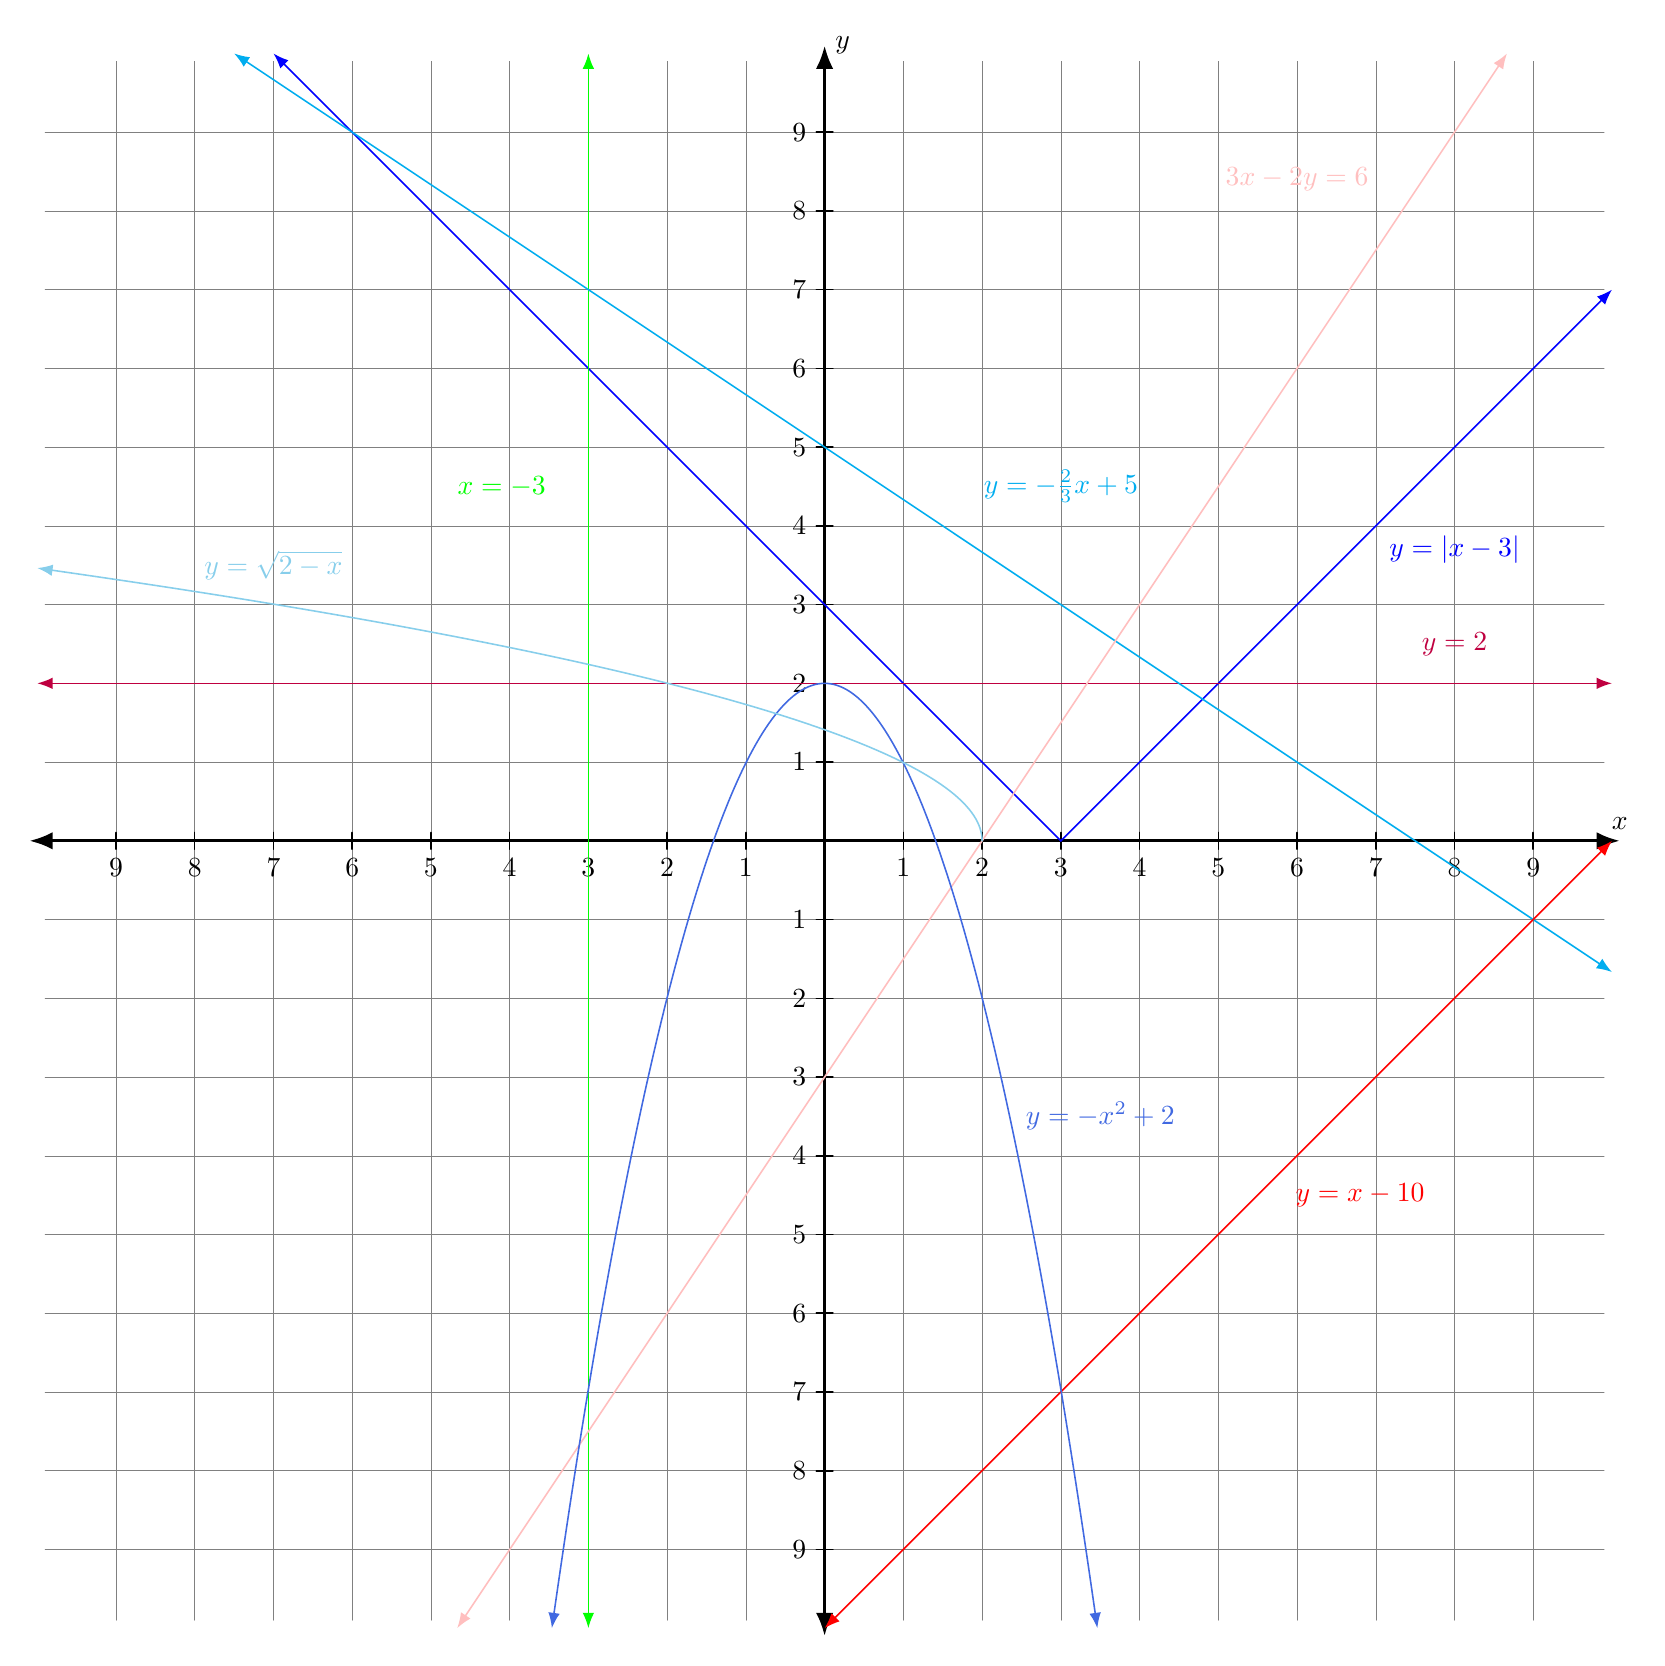
\begin{tikzpicture}[%
    >=Latex,
    line width=0.2mm,
    line cap=round
]
    % Draw a grid.
    \draw[style=help lines] (-9.9, -9.9) grid (9.9, 9.9);

    % Axes:
    \begin{scope}[very thick]
        \draw[<->] (-10.1,  0.0) to (10.1, 0.0) node [above] {$x$};
        \draw[<->] ( 0.0, -10.1) to (0.0, 10.1) node [right] {$y$};
    \end{scope}

    % Axes labels.
    \foreach\n in{1, 2, 3, 4, 5, 6, 7, 8, 9}{%
        \draw (\n,  3pt) to ( \n, -3pt) node [below] {$\n$};
        \draw (-\n, 3pt) to (-\n, -3pt) node [below] {$\minus\n$};
        \draw (3pt,  \n) to (-3pt,  \n) node [left]  {$\n$};
        \draw (3pt, -\n) to (-3pt, -\n) node [left]  {$\minus\n$};
    }
    \draw[draw=blue, <->] (-7, 10) to (3,0) to (10, 7);
    \draw[draw=green, <->] (-3, -10) to (-3, 10);
    \draw[draw=purple, <->] (-10,2) to (10,2);
    \draw[draw=cyan, <->] (-7.5, 10) to (10, -1.667);
    \draw[draw=pink, <->] (-4.6666, -10) to (8.6666, 10);
    \draw[draw=red, <->] (0, -10) to (10, 0);
    \draw[draw=RoyalBlue, <->] (-3.4641, -10) parabola bend (0, 2) (3.4641, -10);
    \draw[rotate=90, shift={(0,-2)}, SkyBlue, ->] (0, 0) parabola bend (0, 0) (3.4641, 12);
        
    \node at (8, 3.7) {$\color{blue}y=|x-3|$};
    \node at (-4.1, 4.5) {$\color{green}x=-3$};
    \node at (8, 2.5) {$\color{purple}y=2$};
    \node at (3, 4.5) {$\color{cyan}{y=-\frac{2}{3}x+5}$};
    \node at (6, 8.4) {$\color{pink}3x-2y=6$};
    \node at (3.5, -3.5) {$\color{RoyalBlue}y=-x^{2}+2$};
    \node at (6.8, -4.5) {$\color{red}y=x-10$};
    \node at (-7, 3.5) {$\color{SkyBlue}y=\sqrt{2-x}$};
  \end{tikzpicture}}
            \caption{The solution to problem \ref{problem:north_shore_exam_graph_everything}.}
            \label{fig:north_shore_graphing_problem}
        \end{figure}
    \subsection{Systems of Equations}
        A system of equations is a set of 2 or more equations involving the same variables. Solving systems of linear equations is one of the main focuses in the study of linear algebra.
        \begin{fexample}{}{}
        \label{example:north_shore_example_of_a_system_of_linear_equations}Consider the following system of linear equations:
        \begin{align*}
            2x+3y&=1\\
            x+6y&=2
        \end{align*}
        Solving this system of equations asks ``Which ordered pairs $(x,y)$ solve both of these equations?" The second equations says that $x=2-6y$. We can substitute this back into the first equation to get $2(2-6y)+3y=1$ which simplifies to $4-9y=1$. The solution to this is $y=\frac{1}{3}$. Solving for $x$, we have $x=2-6y=2-6(\frac{1}{3})=2-2=0$. $(0,\frac{1}{3})$ is a solution.
        \end{fexample}
        We can picture these types of problems graphically as well. For the example above there are two linear equations, which can be represented graphically as lines. A solution to this system can then be interpreted as a point where the two lines intersect. The graph of the two equations in example \ref{example:north_shore_example_of_a_system_of_linear_equations} are shown in Fig.~\ref{fig:north_shore_systems_of_linear_equations}.
        \begin{figure}[H]
            \centering
            \captionsetup{type=figure}
            \documentclass[crop,class=article]{standalone}
%----------------------------Preamble-------------------------------%
\usepackage[dvipsnames]{xcolor}         % Color names.
\usepackage{tikz}                       % Drawing/graphing tools.
\usetikzlibrary{arrows.meta}            % Latex and Stealth arrows.
%--------------------------Main Document----------------------------%
\begin{document}
    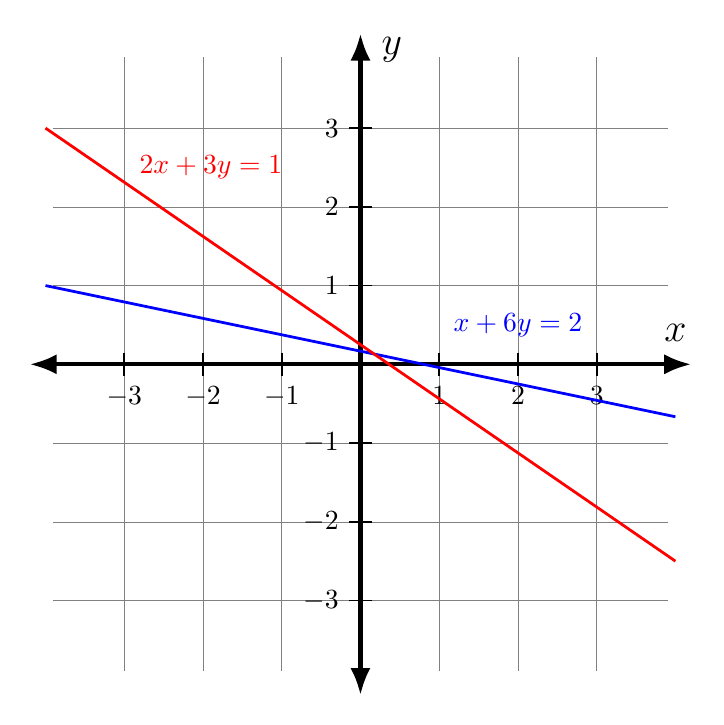
\begin{tikzpicture}[>=latex, line width=1pt]
        \draw[style=help lines] (-3.9, -3.9) grid (3.9, 3.9);
        \begin{scope}[line width=1.5pt, >=Latex, font=\Large]
            \draw[<->] (-4.2, 0) to (4.2, 0);
            \draw[<->] (0, -4.2) to (0, 4.2);
            \node at (4, 0.4) {$x$};
            \node at (0.4, 4) {$y$};
        \end{scope}
        \foreach\x in {-3, -2, -1, 1, 2, 3}
            \draw[shift={(\x,0)}, semithick]
                (0, 0.15) -- (0, -0.15) node[below] {$\x$};
        \foreach\y in {-3, -2, -1, 1, 2, 3}
            \draw[shift={(0, \y)}, semithick]
                (0.15, 0) -- (-0.15, 0) node[left] {$\y$};
        \draw[draw=blue] (-4,1) to (4,-0.666);
        \draw[draw=red] (-4,3) to (4,-2.5);
        \node at (-1.9, 2.5) {$\color{red}2x+3y=1$};
        \node at (2, 0.5) {$\color{blue}x+6y=2$};
    \end{tikzpicture}
\end{document}
            \caption{The graphs of the two equations shown in example \ref{example:north_shore_example_of_a_system_of_linear_equations}.}
            \label{fig:north_shore_systems_of_linear_equations}
        \end{figure}
        Any system of linear equations has 3 possible outcomes: No solutions, one solution, or infinitely many solutions. This makes sense if one considers the few possibilities allowed. Given two parallel lines there will be no solutions for parallel lines never intersect. Given two equations that represent the same line there will be infinitely many solutions, for any point on the line will work. Given two equations for two distinct non-parallel lines there will be only one solution, for such lines can only intersect once.
        \subsubsection{Problems}
        \begin{problem}
        Solve the following system of equations:
        \begin{align*}
            2x-3y&=-12\\
            x-2y&=-9
        \end{align*}
        \end{problem}
        \begin{proof}[Solution]
        Subtracting 2 of the second equation from first equation, we get:
        \begin{equation*}
            (2x-3y)-2(x-2y)=-12-2(-9)
        \end{equation*}
        Which simplifies to $y=6$. The second equation yield $x-2(6)=-9\Rightarrow x=3$. The solution is $(3,6)$
        \end{proof}
        \begin{problem}
        Solve the following system of equations:
        \begin{align*}
            4x+6y&=10\\
            2x+3y&=5
        \end{align*}
        \end{problem}
        \begin{proof}[Solution]
        Dividing both sides of the first equation by 2 gives us the second equation. These equations represent the same line, and there are infinitely many solutions: $y=\frac{5}{3}-\frac{2}{3}x$
        \end{proof}
        \begin{problem}
        Solve the following system of equations:
        \begin{align*}
            x+2y&=5\\
            x+2y&=7
        \end{align*}
        \end{problem}
        \begin{proof}[Solution]
        Let $z=x+2y$. Then $z=5$ and $z=7$. But this is impossible, for $5\ne 7$. No solutions.
        \end{proof}
        \begin{problem}
        \begin{align*}
            2x-3y&=-4\\
            2x+y\phantom{3}&=\phantom{-}4
        \end{align*}
        \end{problem}
        \begin{proof}[Solution]
        Subtracting the first equation from the second gives us $4y=8\Rightarrow y=2$. But then from the first equation we obtain $2x=3(2)-4=2\Rightarrow x=1$. The solution is $(1,2)$.
        \end{proof}
    \subsection{Radicals}
        To simplify expressions with radicals we use something called the conjugate of a radical expression. 
        \begin{fdefinition}
        The conjugate of a rational expression $\sqrt{a}-\sqrt{b}$ is $\sqrt{a}+\sqrt{b}$.
        \end{fdefinition}
        Using the \gls{foil} rule from before, we can obtain the following theorem.
        \begin{ftheorem}{}
            If $a,b\geq 0$, and if $a\ne b$, then
            $\frac{1}{\sqrt{a}-\sqrt{b}}=\frac{\sqrt{a}+\sqrt{b}}{a-b}$
        \end{ftheorem}
        \begin{proof}
        As $a,b\geq 0$ and $a\ne b$, $\frac{1}{\sqrt{a}-\sqrt{b}}$ is well-defined and $\sqrt{a}+\sqrt{b}\ne 0$. But then:
        \begin{align*}
            \tfrac{1}{\sqrt{a}-\sqrt{b}}&=\tfrac{1}{\sqrt{a}-\sqrt{b}}\tfrac{\sqrt{a}+\sqrt{b}}{\sqrt{a}+\sqrt{b}}\\
            &=\tfrac{\sqrt{a}+\sqrt{b}}{(\sqrt{a}-\sqrt{b})(\sqrt{a}+\sqrt{b})}\\
            &=\tfrac{\sqrt{a}+\sqrt{b}}{a-b}&\tag{Thm.~\ref{th:north_shore_difference_of_squares}}
        \end{align*}
        \end{proof}
        \subsubsection{Problems}
        \begin{problem}
        Simplify the following so that there are no radicals in the denominator:
        \begin{enumerate}
        \begin{multicols}{3}
            \item $\sqrt{8}\sqrt{10}$
            \item $\sqrt[4]{\frac{81}{x^4}}$
            \item $\sqrt{\frac{4}{3}}$
            \item $\sqrt{\frac{12}{18}}$
            \item $\sqrt[3]{24x^{3}y^{6}}$
            \item $\frac{\sqrt{3}}{5-\sqrt{3}}$
        \end{multicols}
        \end{enumerate}
        \end{problem}
        \begin{proof}[Solution]
        \
        \begin{enumerate}
        \begin{multicols}{3}
            \item $\sqrt{8}\sqrt{10}=\sqrt{16\cdot 5}=4\sqrt{5}$
            \item $\sqrt[4]{\frac{81}{x^{4}}}=\frac{3}{|x|}$
            \item $\sqrt{\frac{4}{3}}=\frac{2}{\sqrt{3}}=\frac{2\sqrt{3}}{3}$
            \item $\sqrt{\frac{12}{18}}=\frac{2\sqrt{3}}{3\sqrt{2}}=\frac{2\sqrt{2}\sqrt{3}}{6}$
            \item $\sqrt[3]{24x^{3}y^{6}}=2\sqrt[3]{3}xy^{2}$
            \item $\frac{\sqrt{3}}{5-\sqrt{3}}=\frac{\sqrt{3}(5+\sqrt{3})}{5-3}=\frac{5\sqrt{3}+3}{2}$
        \end{multicols}
        \end{enumerate}
        \end{proof}